\documentclass[journal]{IEEEtran}

% --- Math and theorem packages ---
\usepackage{amsmath,amssymb,amsfonts}
\usepackage{amsthm}
% --- Algorithms ---
\usepackage{algorithm}
\usepackage[noend]{algpseudocode}

% --- Other packages ---
\usepackage{array}
\usepackage[caption=false,font=normalsize,labelfont=sf,textfont=sf]{subfig}
\usepackage{textcomp}
\usepackage{stfloats}
\usepackage{url}
\usepackage{verbatim}
\usepackage{graphicx}
\usepackage{cite}
\usepackage{xcolor}
\usepackage{booktabs}
\usepackage{multirow}
\usepackage{tikz}
\usetikzlibrary{arrows,shapes,patterns}
\usepackage{balance}
\usepackage{enumitem}
\usepackage{mdframed}
\usepackage{bm}


\newtheorem{theorem}{Theorem}
\newtheorem{corollary}{Corollary}
\newtheorem{definition}{Definition}
\newtheorem{proposition}{Proposition}


\usetikzlibrary{arrows.meta, positioning, fit, calc}
\newtheorem{remark}{Remark}
%  mathematical commands
\newcommand{\bftheta}{\boldsymbol{\theta}}
\newcommand{\bfphi}{\boldsymbol{\phi}}
\newcommand{\bfvarphi}{\boldsymbol{\varphi}}
\newcommand{\vect}[1]{\bm{#1}}
\newcommand{\field}[1]{\mathbb{#1}}


\begin{document}

\title{Diversity Transforms for OTFS-based LEO Non-Terrestrial Networks}

\author{Chathuranga~M.~Wijerathna~Basnayaka, Haeyoung~Lee, Vishalya P. Sooriarachchi, Pandelis~Kourtessis~and~John~M.~Senior% <-this stops a space
\thanks{Chathuranga~M.~Wijerathna~Basnayaka, Haeyoung~Lee, 
Pandelis~Kourtessis and John~M.~Senior are with the University 
of Hertfordshire, Hatfield, AL10 9AB, United Kingdom. 
Vishalya~P.~Sooriarachchi is with COPELABS, Lus\'{o}fona 
University, Lisbon 1700-097, Portugal. (email: 
c.wijerathna-basnayaka-mudiyanselage@herts.ac.uk, 
h.lee@herts.ac.uk, a22211643@alunos.ulht.pt, 
p.kourtessis@herts.ac.uk, j.m.senior@herts.ac.uk).}}


\markboth{IEEE Internet of Things Journal,~Vol.~XX, No.~XX, April~2026}%
{Basnayaka \MakeLowercase{\textit{et al.}}: Diversity Transforms for OTFS-based LEO Non-Terrestrial Networks }

%\IEEEpubid{0000--0000/00\$00.00~\copyright~2024 IEEE}

\maketitle


\begin{abstract}
Low Earth orbit (LEO) satellite constellations are a key enabler for non-terrestrial networks (NTNs) in sixth-generation (6G) systems. However, achieving high reliability over NTN links for mission-critical applications remains challenging, particularly for high-mobility terminals. Existing transmission diversity techniques based on selection combining or maximal ratio combining (MRC) provide no guaranteed recovery under simultaneous channel outages. Moreover, conventional retransmission schemes in the NTN are incompatible with strict latency constraints in 6G. This paper introduces a diversity transform that integrates forward error correction (FEC) coding with transmission diversity to improve the reliability of orthogonal time frequency space (OTFS)-modulated LEO NTN downlinks. It guarantees block‑erasure recovery up to a prescribed number of subchannels, with residual errors corrected by the outer FEC, thereby eliminating retransmissions. The transform is inserted between the FEC encoder and the modulator, enabling compatibility with various coding schemes and channel models. In this system, a data word is first partitioned into subwords, each independently FEC encoded. A diversity mapper then distributes these encoded subwords across the available subchannels using a binary transform matrix derived from a Reed–Solomon code. This structure guarantees block-erasure recovery whenever a sufficient number of subchannels survive, with residual errors corrected by the outer FEC. An ephemeris-driven reliability prediction framework is developed, combining orbital mechanics, atmospheric models, and a finite-blocklength error probability analysis derived for OTFS transmission over transparent satellite relays. The framework enables proactive outage prediction without channel state information feedback. Simulation results show that the proposed diversity transform provides lower block error rate and reduced latency compared to standalone FEC and retransmission schemes, especially under blockage and high-Doppler conditions characteristic of LEO NTN links.
\end{abstract}
\begin{IEEEkeywords}
Low-Earth-orbit (LEO) satellite communication, non-terrestrial networks (NTNs),
orthogonal time frequency space (OTFS) modulation, diversity transforms,
finite-blocklength analysis.
\end{IEEEkeywords}

\section{Introduction}
\label{sec:introduction}
\IEEEPARstart{M}{ore} than 2.2 billion people, over one quarter of the global population, still lack internet access~\cite{ITU2025Facts}. To bridge this connectivity gap, Low Earth orbit (LEO) satellite constellations have emerged as a promising approach to achieving global connectivity~\cite{Kodheli2021,3GPP38821,Lin2021,Luo24}. However, when LEO satellite communication (SatCom) is used for mission-critical applications such as autonomous vehicles, remote surgery, and industrial control, high reliability and low latency are required~\cite{Azari2022, Nguyen2024, Durisi2016, Basnayaka2026AoI}. Achieving high reliability and low latency over LEO non-terrestrial networks (NTN) links remains a challenge due to highly dynamic channel conditions, including rapid Doppler shifts, long propagation delays, and limited link budget~\cite{11240599}. These challenges are further amplified for high mobility terminals such as high-speed trains, unmanned aerial vehicles (UAVs), and vehicular platforms, where rapid channel variations compound the already severe Doppler shifts induced by LEO orbital motion~\cite{Li2021}. Conventional retransmission schemes such as automatic repeat request (ARQ) and hybrid ARQ (HARQ) are incompatible with the strict latency constraints of mission‑critical applications. Consequently, a retransmission-free approach is necessary to provide high reliability through transmission diversity. Satellite diversity is a well-established countermeasure against shadowing and blockage~\cite{Buzzi2023,596901,11299592,Wang2003}, eliminating the need for retransmission schemes. Multi-connectivity, which creates a channel comprising multiple independently fading subchannels, is inherently capable of supporting transmission diversity. However, current multi-connectivity designs combine independently received signal replicas through selection combining (SC) or maximal ratio combining (MRC)~\cite{li2024multiple}. These approaches offer statistical diversity gains but cannot guarantee data recovery when several subchannels are simultaneously lost, a scenario that frequently arises due to the correlated elevation-angle dynamics of co-visible LEO satellites at low elevations.


To overcome this limitation, a more structured approach is needed, one that guarantees recovery from block erasures under any pattern affecting up to a prescribed number of subchannels. The diversity transform framework meets this need by inserting a linear mixing layer between the forward error correction (FEC) encoder and the physical subchannels, enabling algebraic recovery of the original message whenever a sufficient number of subchannels survive~\cite{Arikan2025_patent,545895}. The diversity transform is implemented using a rectangular binary matrix whose algebraic structure ensures recoverability under prescribed outage patterns. The transform outputs are formed as linear combinations of the encoded subwords according to the rows of this matrix. A key architectural feature of this system is the modular separation between error correction and diversity functions, providing well‑defined interfaces to the encoder and the channel. This allows a given diversity transform to be composed with any FEC scheme, including low-density parity-check (LDPC), turbo, or polar codes, and any compatible channel model without requiring cross-layer redesign. The algebraic strength of this framework lies in its full rank criterion. When a subchannel outage erases an entire group of transform outputs, the data word remains recoverable if and only if the surviving submatrix retains full row rank. Unlike statistical combining methods, which degrade under correlated outages, the full-rank criterion provides a strict algebraic guarantee: any outage pattern within the transform’s design space enables recovery from block erasures.
The diversity transform is constructed based on a predicted erasure
pattern derived from per subchannel reliability analysis in this paper. In satellite communication systems, obtaining accurate channel state information (CSI) feedback is difficult due to high mobility and long propagation delays. Satellites also use many antenna elements to compensate for large path loss, which significantly increases the CSI overhead~\cite{Wang2025PolarXLMIMO}. Most significantly, CSI feedback mechanisms cannot be used in mission‑critical applications due to stringent latency constraints. Thus, this paper proposes an ephemeris based channel prediction framework~\cite{10902219} to compute the per subchannel reliability scores used for transform selection, thus eliminating the need for CSI feedback from the user equipment.

Although the diversity transform addresses satellite outage protection in a LEO-based SatCom system, the physical layer modulation on each subchannel must mitigate the severe Doppler shifts and multipath effects due to rapid LEO orbital motion, which are further compounded by UE mobility. The resulting doubly selective channel renders conventional orthogonal frequency-division multiplexing (OFDM) unsuitable due to inter-carrier interference from large Doppler spreads~\cite{Li2021}. Orthogonal time frequency space (OTFS) modulation addresses this limitation by mapping symbols onto a delay-Doppler (DD) grid and employing the quasi-static channel structure to achieve full multipath diversity~\cite{Hadani2017,Raviteja2018}. OTFS is therefore adopted as the physical-layer waveform for each subchannel in the proposed LEO-based communication system.

Conventional communication systems rely on long codewords to achieve high reliability. However, mission-critical satellite applications demand short-packet transmission to minimize latency in the presence of large propagation delays \cite{Durisi2016,Basnayaka2022,Polyanskiy2010}. On the other hand, conventional asymptotic information-theoretic models developed for long-packet communication are unsuitable for analysing the block error probability in the short packet regime. Thus, finite-blocklength information theory has been adopted as the analytical framework for short packet communication in SatCom systems~\cite{10609803}. In addition, it is crucial to analyse OTFS based satellite communication systems using finite-blocklength information theory. This is especially important for satellite networks serving high mobility users, where OTFS modulation is employed to overcome the severe Doppler effects induced by LEO orbital motion.

\subsection{Related Works}
\label{sec:related_works}

\par Transmission diversity over multiple independently fading subchannels has been a cornerstone of reliable data recovery in wireless communications for decades~\cite{661038,11202644}.  By transmitting redundant replicas of the information symbol across statistically independent fading branches, combining schemes such as SC and MRC effectively mitigate the probability of simultaneous deep fades, thereby enhancing link reliability~\cite{Cacuango2025}. Beyond SC and MRC, recent studies have explored more advanced receiver-side diversity strategies, including space-time block coded combining for multi-satellite systems~\cite{Singh2024}, model-driven deep learning detectors that learn optimal signal combining from data~\cite{He2020DL, Hu2023DL}, and adaptive deep learning-based receiver architectures that learn to handle time-varying channel conditions without explicit mathematical models~\cite{Doha2025}. These techniques improve combining performance under complex channel conditions through learned or structured receiver processing. However, all of these approaches operate at the receiver side and combine multiple copies of the same transmitted signal. In contrast, the diversity transform proposed in this work operates at the transmitter side by algebraically mixing different coded content across subchannels prior to transmission, thereby providing a deterministic erasure recovery guarantee that receiver-side combiners alone cannot provide when an entire subchannel is erased.


On the other hand, several studies have introduced diversity-guaranteeing coding over non-ergodic fading or block fading channels~\cite{Ju2022,5550477,6069883}. For example, polar codes have been combined with interleaving and multi-kernel constructions to enhance resilience over block fading channels~\cite{Ju2022,Niu2021,Mori2010}. However, none of these methods offers an explicit algebraic condition for guaranteed recovery. They also fail to provide strict worst-case guarantees against particular outage patterns. Recently, an error correction coding scheme that integrates transmission diversity was introduced in~\cite{Arikan2025_patent}. The framework proposed in~\cite{Arikan2025_patent} guarantees full message recovery from any sufficient subset of surviving subchannels under block-aligned erasures, requiring no interleavers. Nevertheless, it has not been applied to any specific channel model or communication system, and its iterative receiver architecture introduces additional decoding latency.

In addition, advanced waveforms have been proposed for SatCom to address its 
unique challenges, such as severe Doppler shifts \cite{11373535}. Among these, OTFS modulation 
has emerged as a particularly promising waveform for LEO SatCom~\cite{Shi2022, 
Ren2025, 9508932,11373535}. A key property of OTFS is that it transforms the time-varying 
channel into a two-dimensional representation in the DD domain, 
where all transmitted symbols undergo an identical channel gain~\cite{9904495}. Consequently, OTFS mitigates the severe Doppler effects caused by high relative velocities between satellites and ground users, delivering improved robustness and reliability over traditional schemes such as OFDM. 
Existing studies have demonstrated these advantages in LEO satellite systems, showing that OTFS exhibits strong resilience under high mobility conditions typical of LEO orbits~\cite{Shi2022, Shi2024_Network}. Moreover, coded OTFS schemes achieve full multipath diversity when the DD grid dimensions exceed the number of resolvable paths, thereby providing substantial diversity gains and enhanced error performance~\cite{Li2021}.

Despite these advantages, OTFS-modulated systems for low‑latency applications introduce additional design challenges, as existing outage performance analyses of OTFS~\cite{Shi2022} assume infinite blocklength, an assumption unsuitable for mission‑critical communications~\cite{10529933}. Finite‑blocklength analysis has received considerable attention in the literature, motivated by the short‑packet transmission requirements~\cite{Durisi2016, Basnayaka2022,9528059} of modern mission‑critical communications. For example, non‑asymptotic bounds on achievable rate at finite-blocklength were established in~\cite{Polyanskiy2010}, with extensions to quasi‑static fading channels in~\cite{Yang2014, Durisi2016, Makki2014}. In LEO NTN systems, short‑packet transmission is further constrained by the limited OTFS frame dimensions imposed by coherence time and end‑to‑end latency budgets~\cite{10847811}, making finite‑blocklength theory a primary design consideration rather than an asymptotic blocklength assumption as in conventional wireless systems~\cite{Basnayaka2022,Makki2014}. Thus, investigating the block error rate (BLER) of OTFS under finite-blocklength is necessary to align theoretical analysis with practical implementation of this modulation scheme in LEO NTNs. Finite‑blocklength outage bounds for OTFS were derived in~\cite{Zhang2024} by reformulating the problem as an equivalent parallel AWGN channel. However, that analysis is restricted to generic terrestrial channels; it does not capture the fading characteristics of LEO NTN links, the relay structure, or how the resulting BLER expressions connect to a diversity transform design. To the best of the authors’ knowledge, no existing work has analysed the diversity transform in the finite‑blocklength regime, and its performance has not been evaluated within a practical communication system.

\subsection{Motivations and Contributions}
\label{sec:motivations_contributions}
The literature survey reveals the following critical gaps. First, existing multi-satellite diversity techniques rely on statistical combining and cannot
  guarantee data recovery under arbitrary block-erasure patterns. Second, no algebraic framework exists for constructing diversity transforms for SatCom
  systems. Furthermore, very limited work has been conducted on diversity-transform-supported error correction in wireless communications, and no prior work has analysed the performance of such error correction schemes in a practical setting compared with existing standalone FEC systems. Third, no
  finite-blocklength BLER analysis exists for OTFS based SatCom systems under Rician fading. While the algebraic framework for block-erasure recovery was introduced in~\cite{Arikan2025_patent}, no analysis was provided for any specific channel model or communication system. This paper addresses these gaps by
  developing a diversity transform architecture for LEO based SatCom. The main contributions are as follows:
\begin{itemize}
\item \textit{Diversity Transform for NTN Communications:}
A diversity transform is introduced for OTFS modulated LEO NTN 
systems, and a construction mechanism derived from Reed--Solomon 
codes is presented. This design guarantees recovery from block erasures whenever a sufficient number of subchannels survive, as established in Theorem~\ref{thm:block_mds}.
\item \textit{Finite blocklength BLER Analysis for OTFS based 
SatCom Systems:}
The finite-blocklength BLER is derived for OTFS modulation over 
a transparent satellite relay, accounting for the cascaded relay 
structure and OTFS enabled multipath diversity under Rician fading. 
Tractable closed-form approximations are provided under 
dominant-LOS, high-SNR, and pure Rayleigh fading conditions, 
and the derived expressions are used to compute per subchannel 
reliability scores for the ephemeris based outage prediction 
framework.
\item \textit{Ephemeris-Driven Outage Prediction:}
An ephemeris-driven reliability prediction framework is developed 
that combines orbital mechanics, atmospheric models, and the 
derived finite-blocklength BLER to compute per subchannel 
reliability scores without requiring CSI 
feedback. Subchannels predicted to experience outage are modelled 
as block erasures in the diversity transform domain, enabling the 
diversity transform to be proactively designed against the 
predicted worst-case erasure patterns while maintaining the erasure-recovery guarantee.  In addition, the robustness of the framework to prediction imperfections is analysed through a log-normal perturbation model that captures ephemeris errors, UE location uncertainty, and atmospheric model mismatch.
\item \textit{FEC Code Integration with Diversity Transform:}
A scheme to combine FEC with transmission diversity for NTN communications is introduced. Polar codes are adopted as the FEC component, and the combined polar diversity generator matrix has a Kronecker-product structure, 
forming a single rectangular code. 
\item \textit{Latency and Reliability Analysis of Diversity Transform:}
We derive an overall BLER expression for the proposed diversity-transform architecture that accounts for both the irrecoverable erasure event and the residual FEC decoding error on surviving subchannels. We further prove that the minimum OTFS frame blocklength required to achieve a target system reliability decreases monotonically with the number of subchannels and the maximum distance separable (MDS) minimum distance (Corollary~\ref{cor:latency_reduction}).  In addition, we characterise the impact of prediction uncertainty on both system BLER and transmission latency under imperfect subchannel reliability prediction.
\end{itemize}
\subsection{Organisation}
\label{sec:organisation}
The rest of the paper is organised as follows.
Section~\ref{sec:system_model} presents the system model for the LEO-based
NTN communication system, the channel model, and the OTFS modulation scheme
for the SatCom system.
Section~\ref{sec:reliability_analysis} develops the finite-blocklength BLER
analysis and the ephemeris-driven outage prediction mechanism for this system.
Section~\ref{sec:diversity_transform} introduces the diversity transform
layer, the construction of the diversity transform using MDS codes, and the integration with polar codes as the FEC component.
Section~\ref{sec:results} presents numerical results and performance
evaluations under realistic LEO NTN channel conditions. Finally,
Section~\ref{sec:conclusion} concludes the paper.

\textbf{Notation:} (i) Unless otherwise stated, boldface lower-case 
letters denote vectors, and regular letters denote scalars and random 
variables. (ii) $\mathbb{F}_q$ denotes the finite field of order $q$. 
(iii) For a matrix $G$ and index set $J$, $G(J)$ denotes the submatrix 
formed by the columns indexed by $J$, and $G(:,j)$ denotes the $j$th 
column. (iv) $\otimes$ denotes the Kronecker product. (v) 
$Q(\cdot)$ denotes the Gaussian $Q$-function and $Q^{-1}(\cdot)$ its 
inverse. (vi)  $\delta(\cdot)$ denotes the Dirac delta function. 
(vii) $\mathbb{E}[\cdot]$ denotes the expectation operator, and 
$\mathcal{CN}(0,\sigma^2)$ denotes a circularly symmetric complex 
Gaussian distribution with variance $\sigma^2$. (viii) Logarithms
are base-2 unless otherwise stated. (ix) $\Phi(\cdot)$ denotes the standard normal cumulative distribution function. Table~\ref{tab:notation} summarises the key system-level symbols used throughout the paper.

\begin{table}[t]
\centering

\caption{Key Notation}
\label{tab:notation}
\begin{tabular}{@{}cl@{}}
\toprule
\textbf{Symbol} & \textbf{Description} \\
\midrule
$n$ ($= N_{\text{serv}}$) & Number of physical subchannels (serving satellites) \\
$n_{\mathrm{s}}$ & RS code length (number of field-symbol blocks) \\
$k_{\mathrm{c}}$ & RS code dimension (minimum surviving blocks) \\
$m$ & Extension degree of $\mathbb{F}_{2^m}$ \\
$d_{\min}$ & MDS minimum distance ($= n_{\mathrm{s}} - k_{\mathrm{c}} + 1$) \\
$\varrho$ & Number of encoder subwords ($= k_{\mathrm{c}} m$) \\
$n_{\text{out}}$ & Number of diversity transform outputs ($= n_{\mathrm{s}} m$) \\
$G_{\mathrm{DIV}}$ & Binary diversity transform matrix ($\varrho \times n_{\text{out}}$) \\
$N_{\mathrm{D}}, M_{\mathrm{D}}$ & OTFS Doppler and delay grid dimensions \\
$n_c$ & Channel-coding (polar codeword) blocklength \\
$(N, K)$ & Polar code length and information bits \\
$R_c$ & Polar code rate ($= K/N$) \\
$L$ & SCL decoder list size \\
$\epsilon_i^{\mathrm{E2E}}$ & Per-subchannel end-to-end BLER \\
$\epsilon_{\mathrm{sys}}$ & Overall system BLER \\
$f_{\max}$ & Maximum tolerable subchannel failures ($= n - k_{\mathrm{c}}$) \\
$\gamma_i^{\mathrm{c}}$ & Combined end-to-end SNR of subchannel $i$ \\
$P_{\mathrm{total}}$ & Total transmit power \\
$T_{\Delta}$ & Total system latency \\
$\epsilon_{\mathrm{th}}$ & Erasure declaration threshold \\
$\mathcal{E}_{\mathrm{robust}}$ & Predicted erasure family \\
$\mathcal{A}$ & Transform-output-to-subchannel assignment \\
$G_{\mathrm{POL}}$ & Polar code generator matrix \\
$\sigma_p$ & Prediction error standard deviation (dB) \\
$\rho_{\mathrm{blk}}$ & Blockage correlation parameter \\
$\delta_i$ & Prediction error of subchannel $i$ \\
$\check{\gamma}_i^{\mathrm{E2E}}$ & Observed (mismatched) end-to-end SNR of subchannel $i$\\
$\check{\epsilon}_i^{\mathrm{E2E}}$ & Per-subchannel BLER under imperfect prediction \\
$\check{\epsilon}_{\mathrm{sys}}$ & System BLER under imperfect prediction \\
\bottomrule
\end{tabular}
\end{table}

\section{System Model}
\label{sec:system_model}
We consider a LEO SatCom system in which a constellation of satellites 
provides continuous downlink coverage to a moving user equipment (UE) 
on the ground, with connectivity enabled via a gateway station (GS), 
as illustrated in Fig.~\ref{fig:intro_leo_ntn}. Let 
$k \in \{\mathrm{G},\mathrm{S}\}$ denote a transmitting network node, 
corresponding to the gateway station (GS) or a satellite (S), and let 
$\ell \in \{\mathrm{S},\mathrm{U}\}$ denote the corresponding receiving 
node. At any given time, the UE is simultaneously served by a subset of 
$N_{\text{serv}} \ge 1$ LEO satellites using a multi-connectivity 
protocol to realise satellite diversity. For each $k$--$\ell$ link of subchannel~$i$, the instantaneous slant 
range and LOS direction vector are given by 
$d_{i,k\ell}(t) = \|\vect{r}_{i,k}(t) - \vect{r}_{i,\ell}(t)\|$ and 
$\vect{k}_{i,k\ell}(t) = (\vect{r}_{i,k}(t) - 
\vect{r}_{i,\ell}(t))/d_{i,k\ell}(t)$, respectively, where 
$\vect{r}_{i,k}(t)$ and $\vect{r}_{i,\ell}(t)$ denote the position 
vectors. The elevation angle of satellite~$i$ 
as observed at node $\ell$ is given by 
$\epsilon_{i,k\ell}(t)=\arcsin\!\bigl(\vect{k}_{i,k\ell}(t) \cdot 
\vect{e}_{\mathrm{vert},\ell}\bigr)$, where 
$\vect{e}_{\mathrm{vert},\ell}$ denotes the local zenith unit vector. Downlink connectivity is realized through $n = N_{\text{serv}}$ parallel subchannels. Each subchannel $i \in \{1,\ldots,n\}$ corresponds to a complete end-to-end path through a distinct satellite $i$, incorporating both the feeder link and the access link. Each subchannel operates as a frequency-separated OTFS 
carrier, and the spatial separation of satellites ensures statistically 
independent propagation across subchannels. The diversity transform layer is implemented at the gateway station. The source bitstream is first partitioned into $\varrho$ information 
subwords, each of which is independently encoded by a FEC encoder to produce $\varrho$ parallel codewords, 
which are then linearly transformed into $n_{\text{out}} > \varrho$ 
redundant outputs using a binary diversity matrix 
$\mathbf{G}_{\mathrm{DIV}} \in \mathbb{F}_2^{\varrho \times n_{\text{out}}}$. The resulting $n_{\text{out}}$ transform outputs are mapped onto the $n$ physical subchannels according to a fixed assignment $\mathcal{A} = (A_1,\ldots,A_n)$, where $n = N_{\text{serv}}$ and each subchannel carries $|A_i| = m$ transform outputs corresponding to one field-symbol block, so that $n_{\text{out}} = n \cdot m$. These 
transform outputs are OTFS modulated at the gateway and forwarded to the corresponding satellites via the feeder links. Each satellite employs a 
transparent (bent-pipe) payload that amplifies and frequency-converts the 
received signal without demodulation or decoding, then retransmits on the access 
link toward the UE. On each subchannel, the transmitted symbols are arranged on an $N_D \times M_D$ DD grid and modulated using OTFS. An ephemeris-driven open-loop predictor is employed to estimate future 
satellite and UE states at time $t + T_{\Delta}$, where $T_{\Delta}$ 
denotes the total system latency. Using the predicted ephemerides and 
large-scale channel states $\tilde{G}_{i,\mathrm{GS}}^{\mathrm{LS}}$ and 
$\tilde{G}_{i,\mathrm{SU}}^{\mathrm{LS}}$, the end-to-end (E2E) effective SNR 
$\tilde{\gamma}_{i}^{\mathrm{E2E}}$ is computed. The finite-blocklength 
error probability is then predicted to estimate the reliability of each 
subchannel~$i$. Subchannels whose BLER $\epsilon_{i}^{\mathrm{E2E}}$ exceeds a threshold $\epsilon_{\mathrm{th}}$ are modelled as block erasures in the diversity transform domain, defining the predicted erasure family of subchannels $\mathcal{E}_{\mathrm{robust}}[k+\Delta]$. The 
diversity transform $\mathbf{G}_{\mathrm{DIV}}$ is constructed to 
guarantee full rank recovery for all patterns in this predicted erasure family, as detailed in Section~\ref{sec:diversity_transform}, ensuring 
recoverability of the $\varrho$ information subwords. Finally, the UE performs single‑pass diversity demapping and FEC decoding to recover the original bitstream.

\begin{figure*}[!ht]
    \centering
    \begin{tikzpicture}[
        >=Stealth,
        font=\normalsize,
        ue/.style={
            draw,
            fill=white,
            rounded corners=2pt,
            minimum width=12mm,
            minimum height=6mm
        },
        gw/.style={
            draw,
            fill=white,
            rounded corners=2pt,
            minimum width=13.5mm,
            minimum height=6mm
        },
        info/.style={
            draw,
            fill=white,
            rounded corners=2pt,
            align=left
        },
        subchannel1/.style={
            thick,
            blue!70,
            dashed
        },
        subchannel2/.style={
            thick,
            red!70,
            dash pattern=on 6pt off 3pt
        },
        subchannel3/.style={
            thick,
            violet!70,
            dash pattern=on 3pt off 2pt
        },
        geoarrow/.style={
            thick,
            black!70
        },
        reflection/.style={
            fill=gray!20,
            draw=gray!50,
            opacity=0.7
        }
    ]

    %----------------- GROUND / EARTH CURVATURE -----------------
    \coordinate (gL) at (-8.0,0);
    \coordinate (gC) at (0,-0.5);
    \coordinate (gR) at (6.0,0);
    \draw[thick,blue!40]
        (gL) to[out=0,in=180] (gC)
             to[out=0,in=180] (gR);
    \node[anchor=north east, font=\normalsize] at (gL) {Earth surface};

    %----------------- UE AND GATEWAY (WITH IMAGES) -----------------
    % UE with image
    \node[anchor=south] (ue) at (-1,-0.9) 
        {\includegraphics[width=2.5cm]{smartphone.png}};
    \node[font=\normalsize, anchor=north] at (ue.south) {UE ($U$)};
    
    % Gateway with image
    \node[anchor=south] (gw) at (-7,-0.10)
        {\includegraphics[width=2.5cm]{gateway.png}};
    \node[font=\normalsize, anchor=west] at (gw.east) {Gateway station};

    %----------------- LEO SATELLITES (REAL IMAGES) -----------------
    % Main LEO satellite (connected to UE)
    \node[inner sep=0pt, anchor=center] (sat1) at (3.5,7.5)
        {\includegraphics[width=1.0cm]{leo_satellite}};
    \node[font=\small, anchor=north] at ($(sat1.west)+(-1.3,0.15)$) {LEO satellite $S_{1}$ };
    
    % Additional LEO satellites (not connected to UE)
    \node[inner sep=0pt, anchor=center] (sat2) at (-2.1,7.5)
        {\includegraphics[width=0.7cm]{leo_satellite}};
     \node[font=\small, anchor=north] at ($(sat2.west)+(-1.3,0.18)$) {LEO satellite $S_{2}$ };
   
    
    \node[inner sep=0pt, anchor=center] (sat4) at (5.5,7)
        {\includegraphics[width=0.7cm]{leo_satellite}}; \node[font=\small, anchor=north] at ($(sat4.west)+(2,0.18)$) { LEO satellite $S_{n}$};

    %----------------- ORBIT ARCS -----------------
    % Main orbit arc (through connected satellite)
    \draw[dashed,gray!60]
        (-5.5,8.0) to[out=10,in=190] (6.5,6.6);
    
    % Additional orbit arcs for other satellites
    \draw[dotted,gray!50]
        (-6.2,7.1) to[out=15,in=195] (5.8,8);
    \draw[dotted,gray!50]
        (-6.0,7) to[out=5,in=185] (7.0,5.5);

    %----------------- REFLECTION OBJECTS -----------------
    % Cloud for sub-channel 2 reflection
    \node[cloud, draw, aspect=2, cloud puffs=10, cloud puff arc=120, 
          fill=white, minimum width=1.5cm, minimum height=1cm] (cloud) at (-2.8,4.4) {};
          \node[cloud, draw, aspect=2, cloud puffs=10, cloud puff arc=120, 
          fill=white, minimum width=1.5cm, minimum height=1cm] (cloud) at (-3.4,4.5) {};
             \node[cloud, draw, aspect=2, cloud puffs=10, cloud puff arc=120, 
          fill=white, minimum width=1.5cm, minimum height=1cm] (cloud) at (-2.5,5) {};
    
    % Building for sub-channel 3 reflection
    \draw[reflection] (4,0) rectangle (5.5,2.5);
    \draw[reflection] (4,2.5) -- (4.2,3) -- (5.3,3) -- (5.5,2.5);
       \draw[reflection] (5.5,0) rectangle (7,3);
    \draw[reflection] (5.5,3) -- (5.7,3.5) -- (6.8,3.5) -- (7,3);

    %----------------- SUB-CHANNEL PATHS -----------------
    % Sub-channel 1: Direct path (blue, dashed)
    \draw[subchannel1, ->] (sat1.south) -- (ue.north);
    \node[font=\normalsize, text=blue!70] at ($(sat1.south)!0.3!(ue.north)$) [xshift=5mm] {Sub-channel 1};
    
    % Sub-channel 2: Reflected by cloud (red, dash pattern)
    \coordinate (reflectionPointCloud) at (-3,4.2); % Reflection point on cloud
    \draw[subchannel2, ->] (sat2.south) -- (reflectionPointCloud);
    \draw[subchannel2, ->] (reflectionPointCloud) -- (ue.north);
    \node[font=\normalsize, text=red!70] at ($(reflectionPointCloud)+(2,1.5)$) {Sub-channel 2};

    
    % Sub-channel 3: Reflected by building (green, different dash pattern)
    \coordinate (reflectionPointBuilding) at (6.6,3.2); % Reflection point on building
    \draw[subchannel3, ->] (sat4.south) -- (reflectionPointBuilding);
    \draw[subchannel3, ->] (reflectionPointBuilding) -- (ue.north);
    \node[font=\normalsize, text=violet!70] at ($(reflectionPointBuilding)+(0.5,2)$) {Sub-channel $n$};

       %----------------- GEOMETRIC QUANTITIES AT UE -----------------
    \draw[geoarrow,->] (ue) -- ++(0,2.5) node[above] {$\mathbf{e}_{\mathrm{vert}}$};
  \draw[geoarrow,->] (ue.north) --  ($(ue)!0.4!(sat1)$) node[above] {$\mathbf{k}_i(t)$} ;
   \node[font=\small] at ($(ue)+(0.35,2)$) {$\epsilon_{i,\mathrm{SU}}(t)$};
   \node[font=\normalsize, align=center] at ($(sat1.south)!0.5!(ue.north)$) 
    [xshift=8mm] {$d_{i,\mathrm{SU}}(t)$};

    % Arc for angle epsilon
    \draw[black!70] (ue.north) ++(0,0.6) arc (90:17:0.5);
    
    %----------------- CONNECTION TO GATEWAY -----------------
    \draw[thick, blue!70, dashed,->]  (gw.north)-- (sat1.south);
 
      \draw[thick, red!70, dashed,->]  (gw.north)-- (sat2.south);
    
      \draw[thick, violet!70, dashed,->]  (gw.north)-- (sat4.south);
    \node[font=\normalsize, text=black!70] at ($(sat4.west)!0.7!(gw.north)$) [xshift=-15mm] {Feeder links};


    \end{tikzpicture}
\caption{LEO SatCom system employing satellite diversity to serve a 
moving UE via $n$ parallel OTFS subchannels}
    \label{fig:intro_leo_ntn}
\end{figure*}

\begin{figure*}[t]
    \centering
    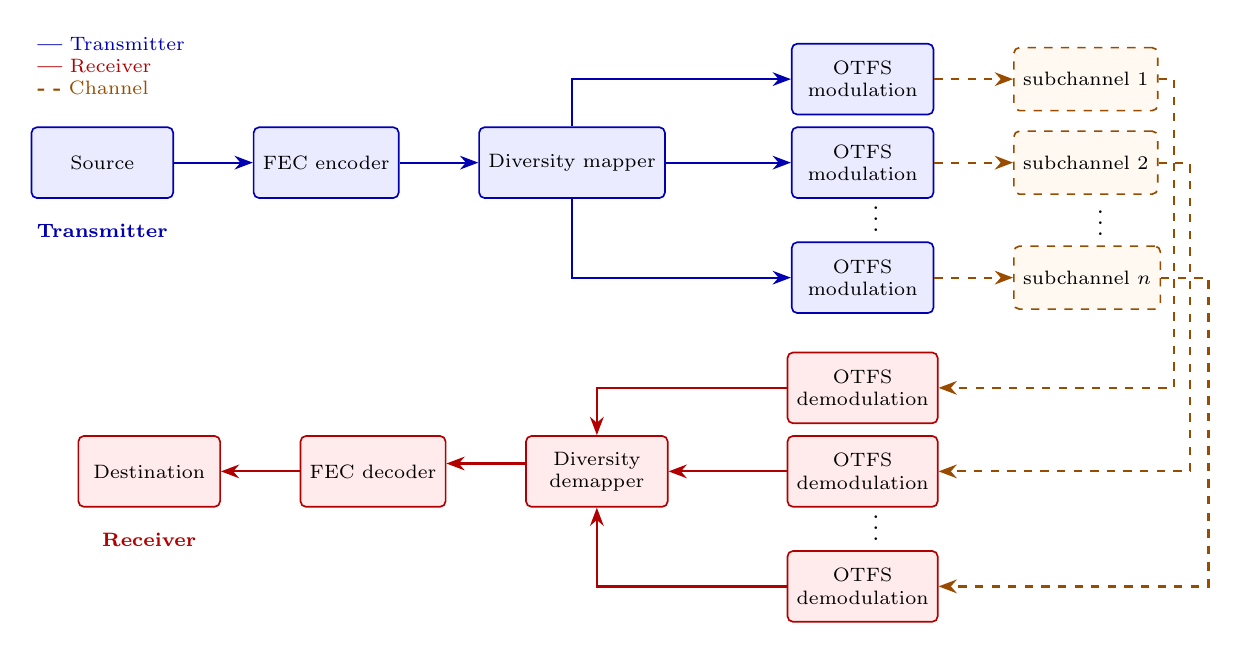
\begin{tikzpicture}[
        >=Stealth,
        node distance = 6mm and 10mm,
        font=\scriptsize,
        block/.style={
            draw=black,
            rectangle,
            rounded corners=2pt,
            minimum height=9mm,
            minimum width=18mm,
            align=center,
            fill=white,
            text=black,
            line width=0.6pt
        },
        txblock/.style={
            draw=blue!70!black,
            rectangle,
            rounded corners=2pt,
            minimum height=9mm,
            minimum width=18mm,
            align=center,
            fill=blue!8,
            text=black,
            line width=0.6pt
        },
        rxblock/.style={
            draw=red!70!black,
            rectangle,
            rounded corners=2pt,
            minimum height=9mm,
            minimum width=18mm,
            align=center,
            fill=red!8,
            text=black,
            line width=0.6pt
        },
        subchan/.style={
            draw=orange!60!black,
            rectangle,
            rounded corners=2pt,
            minimum height=8mm,
            minimum width=16mm,
            align=center,
            fill=orange!5,
            text=black,
            line width=0.6pt,
            dashed
        },
        line/.style={-Stealth, thick, black!60},
        txline/.style={-Stealth, thick, blue!70!black},
        rxline/.style={-Stealth, thick, red!70!black},
        chanline/.style={-Stealth, thick, orange!60!black, dashed}
    ]

    %----------------- TRANSMITTER SIDE -----------------
    \node[txblock] (src) {Source};
    \node[txblock, right=of src] (fec) {FEC  encoder};
    \node[txblock, right=of fec] (div) {Diversity mapper};
    
    %----------------- n PARALLEL PATHS (n=3 shown) -----------------
    \coordinate (path_center) at ([xshift=25mm]div.east);
    
    % Path 1 (top)
    \node[txblock, above=6mm of path_center] (otfs_tx1) {OTFS\\ modulation};
    \node[subchan, right=of otfs_tx1] (chan1) {subchannel 1};
    \node[rxblock, below=30mm of otfs_tx1] (otfs_rx1) {OTFS\\ demodulation};
    
    % Path 2 (middle)
    \node[txblock, at={(path_center)}] (otfs_tx2) {OTFS\\ modulation};
    \node[subchan, right=of otfs_tx2] (chan2) {subchannel 2};
    \node[rxblock, below=30mm of otfs_tx2] (otfs_rx2) {OTFS\\ demodulation};
    
    % Path 3 (bottom)
    \node[txblock, below=10mm of path_center] (otfs_tx3) {OTFS\\ modulation};
     \node[above right=0mm and 0mm of otfs_tx3.north, font=\small] {$\vdots$};
    \node[subchan, right=of otfs_tx3] (chan3) {subchannel $n$};
    \node[above right=0mm and 0mm of chan3.north, font=\small] {$\vdots$};
    \node[rxblock, below=30mm of otfs_tx3] (otfs_rx3) {OTFS\\ demodulation};
    \node[above right=0mm and 0mm of otfs_rx3.north, font=\small] {$\vdots$};
    
  
    

    
    %----------------- RECEIVER SIDE -----------------
    \node[rxblock, left=15mm of otfs_rx2] (demap) {Diversity\\ demapper};
    \node[rxblock, left=of demap] (dec) {FEC decoder};
    \node[rxblock, left=of dec] (sink) {Destination};

    %----------------- DATA FLOW -----------------
    % Transmitter chain
    \draw[txline] (src) -- (fec);
    \draw[txline] (fec) -- (div);
    
    % Split to n parallel paths
    \draw[txline] (div.north) |- (otfs_tx1.west);
    \draw[txline] (div.east) -- (otfs_tx2.west);
    \draw[txline] (div.south) |- (otfs_tx3.west);
    
    % Each path: OTFS mod → channel → OTFS demod
    % Channel paths
    \draw[chanline] (otfs_tx1.east) -- (chan1.west);
    \draw[chanline] (chan1.east) -- ++(2mm,0) |- (otfs_rx1.east);
    
    \draw[chanline] (otfs_tx2.east) -- (chan2.west);
    \draw[chanline] (chan2.east) -- ++(4mm,0) |- (otfs_rx2.east);
    
    \draw[chanline] (otfs_tx3.east) -- (chan3.west);
    \draw[chanline] (chan3.east) -- ++(6mm,0) |- (otfs_rx3.east);
    
    % Merge from n demodulators to demapper
    \draw[rxline] (otfs_rx1.west) -| (demap.north);
    \draw[rxline] (otfs_rx2.west) -- (demap.east);
    \draw[rxline] (otfs_rx3.west) -| (demap.south);
    
    % Receiver chain: bidirectional connection between demapper and decoder (as in the image)
   \draw[rxline] ([yshift=1mm]demap.west) -- ([yshift=1mm]dec.east);
    \draw[rxline] (dec) -- (sink);

    %----------------- LABELS -----------------
    \node[below=2mm of src, font=\scriptsize\bfseries, color=blue!70!black] {Transmitter};
    \node[below=2mm of sink, font=\scriptsize\bfseries, color=red!70!black] {Receiver};
    

    
    %----------------- COLOR LEGEND -----------------
    \node[above right=2mm and 0mm of current bounding box.north west, anchor=north west, 
          font=\scriptsize, align=left, text width=2.5cm] {
          \textcolor{blue!70!black}{\textbf{---} Transmitter}\\
          \textcolor{red!70!black}{\textbf{---} Receiver}\\
          \textcolor{orange!60!black}{\textbf{- -} Channel}
    };

    \end{tikzpicture}
  \caption{Transceiver architecture of the LEO NTN OTFS downlink with diversity mapper and $n$ parallel subchannels.}
    \label{fig:simple_overall_system}
\end{figure*}

\subsection{Channel Model}
\label{sec:channel-model}

Each subchannel $i \in \{1,\ldots,n\}$ represents a complete end-to-end path through satellite~$i$, comprising a gateway--satellite feeder link ($G$--$S_i$) and a satellite--UE access link ($S_i$--$U$) operating in cascade. For both links, the propagation follows a doubly selective  tapped-delay-line (TDL-D) fading model. The complex baseband impulse response of the $k$--$\ell$ link within subchannel~$i$ at time $t$ and delay $\tau$ is given by
\begin{equation}
h_{i,k\ell}(t,\tau) = \sum_{p=0}^{L_{i,k\ell}-1} \alpha_{i,k\ell,p}(t)\, \delta(\tau-\tau_{i,k\ell,p}),
\label{eq:ntn_impulse_response}
\end{equation}
where $L_{i,k\ell}$ denotes the number of resolvable taps, $\tau_{i,k\ell,p}$ is the delay of the $p$th path, and $\alpha_{i,k\ell,p}(t)$ is the corresponding complex tap gain. Each tap gain consists of a large-scale path-loss component and a  small-scale Rician fading term, given by
$ \alpha_{i,k\ell,p}(t) = \sqrt{G_{i,k\ell,\mathrm{LS}}(t) \cdot P_{i,k\ell,p}}\, g_{i,k\ell,p}(t),
$ where $P_{i,k\ell,p}$ is the TDL-D relative tap power satisfying 
$\sum_{p=0}^{L_{i,k\ell}-1} P_{i,k\ell,p} = 1$, and 
$G_{i,k\ell,\mathrm{LS}}(t)$ is the linear large-scale gain. The small-scale fading coefficient is modelled as
\begin{equation}
g_{i,k\ell,p}(t) = \sqrt{\frac{K_{i,k\ell}}{K_{i,k\ell}+1}}\, 
e^{j2\pi f_{D,i,k\ell,p}t} + \sqrt{\frac{1}{K_{i,k\ell}+1}}\, 
w_{i,k\ell,p}(t),
\label{eq:rician_fading}
\end{equation}
where $K_{i,k\ell}$ denotes the Rician factor, $f_{D,i,k\ell,p}$ 
is the Doppler shift of tap $p$, and 
$w_{i,k\ell,p}(t)\sim\mathcal{CN}(0,1)$ is the diffuse multipath 
component. The Doppler shift for each tap is given by
$ f_{D,i,k\ell,p} = \frac{v_{\mathrm{rel},i,k\ell}(t)}{\lambda} 
\cos\theta_{i,k\ell,p}(t),
$
where $v_{\mathrm{rel},i,k\ell}(t)$ is the relative velocity 
between nodes $k$ and $\ell$, $\lambda = c/f_c$ is the carrier 
wavelength, and $\theta_{i,k\ell,p}(t)$ is the angle of arrival 
of the $p$th path. The large-scale path loss aggregates multiple propagation effects  and is expressed as
\begin{equation}
\mathrm{PL}_{i,k\ell,\mathrm{tot}}(t) = \mathrm{PL}_{i,k\ell,\mathrm{FS}}(t) 
+ \mathcal{L}_{i,k\ell}^{\mathrm{atm}}(t) 
+ \mathcal{L}_{i,k\ell}^{\mathrm{blk}}(t),
\label{eq:total_path_loss}
\end{equation}
where $\mathrm{PL}_{i,k\ell,\mathrm{FS}}(t)$ is the free-space path 
loss, $\mathcal{L}_{i,k\ell}^{\mathrm{blk}}(t)$ is the combined 
blockage and shadowing loss, and the aggregate atmospheric attenuation 
is given by $
\mathcal{L}_{i,k\ell}^{\mathrm{atm}}(t) \triangleq 
\mathcal{L}_{i,k\ell}^{\mathrm{gas}}(t) 
+ \mathcal{L}_{i,k\ell}^{\mathrm{cf}}(t) 
+ \mathcal{L}_{i,k\ell}^{\mathrm{rain}}(t),
$
comprising gaseous absorption, cloud and fog attenuation, and rain 
fading contributions. The free-space path loss is given by
$
\mathrm{PL}_{i,k\ell,\mathrm{FS}}(t) = 20\log_{10}\!\left(
\frac{4\pi d_{i,k\ell}(t)}{\lambda}\right),
$ where the slant range $d_{i,k\ell}(t)$ is given by \cite{ippolito2017satellite}
\begin{equation}
d_{i,k\ell}(t) = R_E\biggl( \sqrt{\Bigl(1+\frac{h_{\mathrm{orb}}}{R_E}
\Bigr)^2 -\cos^2\epsilon_{i,k\ell}(t)} -\sin\epsilon_{i,k\ell}(t) 
\biggr),
\label{eq:slant_range}
\end{equation}
with $R_E$ denoting the Earth radius and $h_{\mathrm{orb}}$ the orbital altitude. Gaseous absorption is modelled according to \cite{ITU-R_P676-13} with specific attenuation
$
\gamma_i^{\mathrm{gas}}(t) = \gamma_{\mathrm{O_2}}(f_c,P_{\mathrm{atm}},T_{\mathrm{atm}}) + \gamma_{\mathrm{H_2O}}(f_c,P_{\mathrm{atm}},T_{\mathrm{atm}},\rho_i(t)),
$
where $\gamma_{\mathrm{O_2}}$ and $\gamma_{\mathrm{H_2O}}$ are the oxygen and water-vapour absorption coefficients, respectively, $P_{\mathrm{atm}}$ is the atmospheric pressure, $T_{\mathrm{atm}}$ is the temperature, and $\rho_i(t)$ is the water-vapour density. The total gaseous attenuation along the slant path is then
$
\mathcal{L}_{i,k\ell}^{\mathrm{gas}}(t) = \gamma_i^{\mathrm{gas}}(t)\, \frac{H_{\mathrm{gas}}}{\sin\epsilon_{i,k\ell}(t)},
$
where $H_{\mathrm{gas}}$ is the equivalent atmospheric thickness. Cloud and fog attenuation is computed following~\cite{ITUcloud}, with specific attenuation given by
$\gamma_i^{\mathrm{cf}}(t) = K_l(f_c)\,\mathrm{LWC}_i(t),
$ where $K_l(f_c)$ is the specific liquid-water absorption coefficient and $\mathrm{LWC}_i(t)$ is the liquid-water content in g/m$^3$. The resulting cloud and fog attenuation is
$
\mathcal{L}_{i,k\ell}^{\mathrm{cf}}(t) = \gamma_i^{\mathrm{cf}}(t)\, \frac{H_{\mathrm{cf}}}{\sin\epsilon_{i,k\ell}(t)},
$
where $H_{\mathrm{cf}}$ denotes the cloud-layer thickness. Rain attenuation is modelled according to \cite{ITU-R_P618-14} as
$
\mathcal{L}_{i,k\ell}^{\mathrm{rain}}(t) = \kappa\,R_i(t)^{\beta}\, d_{i,k\ell,\mathrm{rain}}(t),
$
where $R_i(t)$ is the rain rate in mm/h, $\kappa$ and $\beta$ are frequency-dependent attenuation coefficients, and the effective rain path length is given by
$
d_{i,k\ell,\mathrm{rain}}(t) = \frac{H_{\mathrm{rain}} - h_{\mathrm{UE}}}{\sin\epsilon_{i,k\ell}(t)} \cdot r_{i}(t),
$
with $H_{\mathrm{rain}}$ being the rain height, $h_{\mathrm{UE}}$ the UE altitude, and $r_{i}(t)$ the path reduction factor. The blockage and shadowing loss $\mathcal{L}_{i,k\ell}^{\mathrm{blk}}(t)$ is governed by a binary line-of-sight (LOS) indicator $B_{i,k\ell}(t)\in\{0,1\}$, where $B_{i,k\ell}(t)=1$ indicates an unobstructed link and $B_{i,k\ell}(t)=0$ denotes deep blockage. The indicator follows a Bernoulli distribution with $\mathbb{P}[B_{i,k\ell}(t)=1] = P_{\mathrm{LOS}}(\epsilon_{i,k\ell}(t),\xi)$, where $\xi \in \{\mathrm{U}, \mathrm{S}, \mathrm{R}\}$ denotes urban, suburban, or rural environment, respectively. According to \cite{3GPP_TR38811}, the LOS probability is
\begin{equation}
P_{\mathrm{LOS}}(\epsilon,\xi) = \begin{cases} 1, & \epsilon \ge \epsilon_{\mathrm{max}}(\xi), \\[4pt] \exp\!\left(-\dfrac{\epsilon_{\mathrm{max}}(\xi)-\epsilon}{\theta(\xi)}\right), & \epsilon_{\mathrm{min}} \le \epsilon < \epsilon_{\mathrm{max}}(\xi), \\[8pt] P_{\mathrm{base}}(\xi), & \epsilon < \epsilon_{\mathrm{min}}, \end{cases}
\label{eq:los_prob}
\end{equation}
where $\epsilon_{\mathrm{min}}$, $\epsilon_{\mathrm{max}}(\xi)$, $\theta(\xi)$, and $P_{\mathrm{base}}(\xi)$ are environment-specific parameters. Conditioned on the blockage state, the blockage loss is expressed as
\begin{equation}
\mathcal{L}_{i,k\ell}^{\mathrm{blk}}(t) = \begin{cases} \mu_{\mathrm{sh}} + X_{i,k\ell}(t), & B_{i,k\ell}(t)=1, \\[4pt] \mathcal{L}_{\mathrm{deep}}, & B_{i,k\ell}(t)=0, \end{cases}
\label{eq:blockage}
\end{equation}
where $\mu_{\mathrm{sh}}$ is the mean shadowing margin, $X_{i,k\ell}(t)\sim\mathcal{N}(0,\sigma_{\mathrm{sh}}^2)$ models lognormal shadow fading, and $\mathcal{L}_{\mathrm{deep}}$ represents the deep-blockage loss.
The preceding model treats blockage indicators
$\{B_{i,k\ell}(t)\}$ as independent across subchannels. In practice,
co-visible LEO satellites at similar low elevations share a common
obstruction environment, introducing spatial correlation in blockage
events. To capture this effect, we adopt a Gaussian copula model~\cite{Nelsen2006, Ghadi2021}. Let
$\mathbf{Z} = [Z_1, \ldots, Z_n]^\top \sim
\mathcal{N}(\mathbf{0}, \mathbf{R}_{\mathrm{blk}})$,
where the equicorrelation matrix has entries
\begin{equation}
[\mathbf{R}_{\mathrm{blk}}]_{ij} = \begin{cases}
1, & i = j, \\
\rho_{\mathrm{blk}}, & i \neq j,
\end{cases}
\label{eq:corr_matrix_blk}
\end{equation}
with $\rho_{\mathrm{blk}} \in [0,1]$. The blockage indicator of
subchannel~$i$ is then defined as
$B_i = \mathbf{1}\{\Phi(Z_i) \leq P_{\mathrm{LOS}}(\epsilon_i)\}$.
Each subchannel maintains its elevation-dependent marginal
blockage probability
$1 - P_{\mathrm{LOS}}(\epsilon_i)$ from~\eqref{eq:los_prob}, while
$\rho_{\mathrm{blk}}$ controls the degree of spatial correlation:
$\rho_{\mathrm{blk}} = 0$ recovers independent blockage, whereas
$\rho_{\mathrm{blk}} \to 1$ approaches a common-blockage scenario in
which all subchannels tend to be simultaneously obstructed.
The linear large-scale channel gain is obtained from the total path loss according to
$G_{i,k\ell,\mathrm{LS}}(t) = 10^{-\mathrm{PL}_{i,k\ell,\mathrm{tot}}(t)/10}.
$ Based on the large-scale channel characterisation, the instantaneous signal-to-noise ratio (SNR) for the $k$--$\ell$ link of subchannel $i$ is
\begin{equation}
\gamma_{i,k\ell}(t)
= \frac{P_k \mathcal{G}_k G_{i,k\ell,\mathrm{LS}}(t) \mathcal{G}_\ell}
{\sigma_{n,\ell}^2}
|g_{i,k\ell}(t)|^2
\label{eq:snr_generic}
\end{equation}
where $P_k$ is the transmit power at node $k$, $\mathcal{G}_k$ and $\mathcal{G}_\ell$ are the antenna gains at the transmitting and receiving nodes, $\sigma_{n,\ell}^2$ is the noise power at receiving node $\ell$, and $|g_{i,k\ell}(t)|^2$ is the small-scale fading power. The total transmit power $P_{\mathrm{total}}$ is equally split between the gateway and satellite, i.e., $P_G = P_S = P_{\mathrm{total}}/2$. The average SNR follows by taking the expectation of \eqref{eq:snr_generic} over the small-scale fading. Under the Rician model in \eqref{eq:rician_fading}, the normalisation condition $
\mathbb{E}\bigl[|g_{i,k\ell}(t)|^2\bigr] 
= \frac{K_{i,k\ell}}{K_{i,k\ell}+1} + \frac{1}{K_{i,k\ell}+1} = 1
$ is obtained, and the average SNR becomes
\begin{equation}
\bar{\gamma}_{i,k\ell}(t)
= \frac{P_k \mathcal{G}_k G_{i,k\ell,\mathrm{LS}}(t) \mathcal{G}_\ell}
{\sigma_{n,\ell}^2}.
\label{eq:avg_snr_generic}
\end{equation} Under the transparent relay architecture, the satellite employs automatic gain control to maintain constant output power. Consequently, the end-to-end effective SNR for subchannel~$i$ is determined by the cascaded combination of both links. Following the analysis in~\cite{Hasna2003}, this cascaded SNR is given by
\begin{equation}
\gamma_{i}^{\mathrm{E2E}}(t) = \frac{\gamma_{i,\mathrm{GS}}(t) \cdot \gamma_{i,\mathrm{SU}}(t)}{\gamma_{i,\mathrm{GS}}(t) + \gamma_{i,\mathrm{SU}}(t) + 1}.
\label{eq:cascaded_snr}
\end{equation}
This expression captures the noise amplification effect inherent to transparent relaying, where the feeder-link noise is amplified and forwarded along with the desired signal. The average end-to-end SNR can be approximated as
\begin{equation}
\bar{\gamma}_{i}^{\mathrm{E2E}}(t) \approx \frac{\bar{\gamma}_{i,\mathrm{GS}}(t) \cdot \bar{\gamma}_{i,\mathrm{SU}}(t)}{\bar{\gamma}_{i,\mathrm{GS}}(t) + \bar{\gamma}_{i,\mathrm{SU}}(t) + 1}.
\label{eq:avg_cascaded_snr}
\end{equation}
In the high-SNR regime, \eqref{eq:cascaded_snr} simplifies to $\gamma_{i}^{\mathrm{E2E}} \approx \min(\gamma_{i,\mathrm{GS}}, \gamma_{i,\mathrm{SU}})$, indicating that the weaker of the two links dominates the end-to-end performance. The feeder link employs high-gain tracking antennas at both the gateway and satellite, typically operating in Ka-band or Q-band with high antenna gains. Due to the narrow beamwidth and absence of significant scatterers at orbital altitudes, the feeder-link channel shows negligible delay spread ($L_{i,\mathrm{GS}} = 1$) and a dominant LOS component ($K_{i,\mathrm{GS}} \gg 1$). Consequently, the feeder-link SNR is quasi-deterministic:
\begin{equation}
\gamma_{i,\mathrm{GS}}(t) \approx \bar{\gamma}_{i,\mathrm{GS}}(t).
\label{eq:feeder_deterministic}
\end{equation}
 This is consistent with the 3GPP NTN simulation framework in TR~38.821~\cite{3GPP38821}, which treats feeder-link SNR impairments as negligible while retaining only the propagation delay. The service-link channel model in TR~38.811~\cite{3GPP_TR38811} considers only the satellite--UE link, where multipath propagation arises from scattering near the UE.
In contrast, the access link experiences multipath propagation due to scattering in the UE's local environment, yielding $L_i = L_{i,\mathrm{SU}} \geq 1$ resolvable paths. The DD diversity exploited by OTFS modulation therefore arises entirely from the access-link multipath structure. The per-path access-link SNR is
$
\gamma_{i,\mathrm{SU},p}(t) = \bar{\gamma}_{i,\mathrm{SU}}(t) \cdot P_{i,\mathrm{SU},p} \cdot |g_{i,\mathrm{SU},p}(t)|^2,
$ where $P_{i,\mathrm{SU},p}$ is the relative power of the $p$th tap and $|g_{i,\mathrm{SU},p}(t)|^2$ is the corresponding small-scale fading power. OTFS modulation enables the receiver to resolve and coherently combine the $L_i$ access-link paths through DD domain processing. With the transparent relay architecture, the multipath components resolved at the receiver share a common amplified feeder-link noise contribution, since the satellite amplifies and forwards the entire received signal including noise. Consequently, after MRC across the $L_i$ resolved access-link paths, the effective end-to-end SNR is given by \cite{Hasna2003}
\begin{equation}
\gamma_i^{\mathrm{c}}(t) = \frac{\bar{\gamma}_{i,\mathrm{GS}}(t) \cdot \gamma_{i,\mathrm{SU}}^{\mathrm{MRC}}(t)}{\bar{\gamma}_{i,\mathrm{GS}}(t) + \gamma_{i,\mathrm{SU}}^{\mathrm{MRC}}(t) + 1},
\label{eq:combined_snr_full}
\end{equation}
where $
\gamma_{i,\mathrm{SU}}^{\mathrm{MRC}}(t) = \sum_{p=0}^{L_i-1} \gamma_{i,\mathrm{SU},p}(t)
$
denotes the MRC-combined access-link SNR. This formulation accounts for the correlated feeder-link noise across all resolved taps while the independent access-link noise contributions add incoherently under MRC. In the typical operating regime where the feeder link employs high-gain tracking antennas and operates with substantially higher SNR than the access link, i.e., $\bar{\gamma}_{i,\mathrm{GS}} \gg \gamma_{i,\mathrm{SU}}^{\mathrm{MRC}}$, the cascaded expression simplifies to
\begin{IEEEeqnarray}{rCl}
\gamma_i^{\mathrm{c}}(t) &\approx& \gamma_{i,\mathrm{SU}}^{\mathrm{MRC}}(t) = \sum_{p=0}^{L_i-1} \gamma_{i,\mathrm{SU},p}(t) \nonumber\\
&=& \bar{\gamma}_{i,\mathrm{SU}}(t) \sum_{p=0}^{L_i-1} P_{i,\mathrm{SU},p} \cdot |g_{i,\mathrm{SU},p}(t)|^2.
\label{eq:combined_snr_approx}
\end{IEEEeqnarray} Under the dominant-LOS approximation ($K_{i,\mathrm{SU},0} \gg 1$), which is typical for LEO satellite channels~\cite{3GPP_TR38811}, the first tap contributes a quasi-deterministic SNR
\begin{equation}
\gamma_{i,0}^{\mathrm{det}} = \bar{\gamma}_{i,\mathrm{SU}}(t) \cdot P_{i,\mathrm{SU},0},
\label{eq:los_deterministic}
\end{equation}
while the remaining $L_i - 1$ non-LOS (NLOS) paths exhibit Rayleigh fading ($K_{i,\mathrm{SU},p} = 0$ for $p \geq 1$). The aggregate NLOS component
\begin{equation}
\gamma_i^{\mathrm{NLOS}}(t) = \bar{\gamma}_{i,\mathrm{SU}}(t) \sum_{p=1}^{L_i-1} P_{i,\mathrm{SU},p} \cdot |g_{i,\mathrm{SU},p}(t)|^2
\label{eq:nlos_aggregate}
\end{equation}
follows a gamma distribution with shape parameter $L_i - 1$ and scale parameter $\hat{\gamma}_{i,\mathrm{NLOS}}$, where $\hat{\gamma}_{i,\mathrm{NLOS}} = \bar{\gamma}_{i,\mathrm{SU}}(t) \cdot P_{\mathrm{NLOS}} / (L_i - 1)$ and $P_{\mathrm{NLOS}} = \sum_{p=1}^{L_i-1} P_{i,\mathrm{SU},p} = 1 - P_{i,\mathrm{SU},0}$. The combined SNR after MRC is therefore
\begin{equation}
\gamma_i^{\mathrm{c}}(t) = \gamma_{i,0}^{\mathrm{det}} + \gamma_i^{\mathrm{NLOS}}(t),
\label{eq:combined_snr_final}
\end{equation}
which follows a shifted gamma distribution with a deterministic offset $\gamma_{i,0}^{\mathrm{det}}$ and a random component $\gamma_i^{\mathrm{NLOS}}(t)$. The total average SNR satisfies the power budget
$\bar{\gamma}_i^{\mathrm{c}} \approx \gamma_{i,0}^{\mathrm{det}} + (L_i-1)\hat{\gamma}_{i,\mathrm{NLOS}} \approx \bar{\gamma}_{i,\mathrm{SU}}(t)$,
under the strong-feeder-link approximation, where noise amplification in the transparent relay becomes negligible.\footnote{Under the parameters in Table~\ref{tab:sim_params}, the ratio $\bar{\gamma}_{i,\mathrm{GS}}/\bar{\gamma}_{i,\mathrm{SU}}$ exceeds 39~dB. According to ITU-R P.618~\cite{ITU-R_P618-14}, Ka-band rain attenuation at 99.9\% link availability for mid-latitude gateway sites is typically 5--12~dB, which reduces this margin to approximately 27--34~dB, well above the 10~dB threshold at which the approximation begins to degrade. The sensitivity of the subchannel BLER to reduced $\bar{\gamma}_{i,\mathrm{GS}}/\bar{\gamma}_{i,\mathrm{SU}}$ is quantified in Fig.~\ref{fig:prop1_validation}.}
\subsection{OTFS Modulation}
\label{sec:otfs}
This subsection presents the OTFS modulation framework that leverages the DD channel structure to achieve diversity across the $L_i$ resolvable paths.  OTFS modulation is performed at the gateway station, and the modulated signal propagates through the cascaded feeder--satellite--access path, characterised by the end-to-end SNR in \eqref{eq:cascaded_snr}, to the UE where OTFS demodulation is performed. On each physical subchannel~$i$, OTFS modulation maps information symbols onto a two-dimensional DD grid of size $N_{\mathrm{D}} \times M_{\mathrm{D}}$, where $N_{\mathrm{D}}$ and $M_{\mathrm{D}}$ represent the numbers of Doppler and delay bins, respectively. Let $x[u,v]$, with $u = 0,\ldots,N_{\mathrm{D}}-1$ and $v = 0,\ldots,M_{\mathrm{D}}-1$, denote the quadrature amplitude modulation (QAM) symbols placed on this grid; here we adopt quadrature phase shift keying (QPSK).  The inverse symplectic finite Fourier transform (ISFFT) maps these DD domain symbols into the time--frequency domain according to
\begin{equation}
X[p,q] = \frac{1}{\sqrt{N_{\mathrm{D}}M_{\mathrm{D}}}} \sum_{u=0}^{N_{\mathrm{D}}-1} \sum_{v=0}^{M_{\mathrm{D}}-1} x[u,v]\, e^{j2\pi\left(\frac{pu}{N_{\mathrm{D}}} - \frac{qv}{M_{\mathrm{D}}}\right)},
\label{eq:isfft}
\end{equation}
for $p = 0,\ldots,N_{\mathrm{D}}-1$ and $q = 0,\ldots,M_{\mathrm{D}}-1$, where $p$ and $q$ denote the discrete time and frequency indices, respectively. The continuous-time transmit signal at the gateway is subsequently obtained via the Heisenberg transform as
\begin{equation}
s(t) = \sum_{p=0}^{N_{\mathrm{D}}-1} \sum_{q=0}^{M_{\mathrm{D}}-1} X[p,q]\,g_{\mathrm{tx}}(t-pT_{\mathrm{sym}})\, e^{j2\pi q \Delta f (t-pT_{\mathrm{sym}})},
\label{eq:tx_signal}
\end{equation}
where $g_{\mathrm{tx}}(\cdot)$ is the transmit pulse-shaping function, $T_{\mathrm{sym}}$ is the OTFS symbol duration, and $\Delta f$ is the subcarrier spacing satisfying the orthogonality condition $\Delta f \cdot T_{\mathrm{sym}} = 1$. At the UE receiver, OTFS demodulation is performed by applying the Wigner transform followed by the symplectic finite Fourier transform (SFFT). The DD domain received symbols are obtained as
\begin{equation}
y_{i}[u,v] = \frac{1}{\sqrt{N_{\mathrm{D}}M_{\mathrm{D}}}} \sum_{p=0}^{N_{\mathrm{D}}-1} \sum_{q=0}^{M_{\mathrm{D}}-1} Y_{i}[p,q]\, e^{-j2\pi\left(\frac{pu}{N_{\mathrm{D}}} - \frac{qv}{M_{\mathrm{D}}}\right)},
\label{eq:sfft}
\end{equation}
where $Y_{i}[p,q]$ denotes the time--frequency domain received samples after matched filtering. Under standard pulse-shaping and sampling assumptions, the DD input--output relation for subchannel~$i$ can be expressed in discrete form as
\begin{IEEEeqnarray}{rCl}
y_{i}[u,v] &=& \sum_{u'=0}^{N_{\mathrm{D}}-1} \sum_{v'=0}^{M_{\mathrm{D}}-1} h_{i}^{\mathrm{E2E}}\!\left[(u-u')_{N_{\mathrm{D}}}, (v-v')_{M_{\mathrm{D}}}\right] \nonumber\\
&& \times\, x[u',v'] + w_{i}[u,v]
\label{eq:dd_io}
\end{IEEEeqnarray}
where $(\cdot)_{N_{\mathrm{D}}}$ and $(\cdot)_{M_{\mathrm{D}}}$ denote modulo-$N_{\mathrm{D}}$ and modulo-$M_{\mathrm{D}}$ operations, respectively, and $w_{i}[u,v] \sim \mathcal{CN}(0, \sigma_{w,i}^2)$ is the effective noise. Under the transparent relay architecture, the effective noise consists of access-link thermal noise and amplified feeder-link noise. When the feeder link dominates, i.e., $\bar{\gamma}_{i,\mathrm{GS}} \gg \bar{\gamma}_{i,\mathrm{SU}}$, the amplified feeder-link noise becomes negligible, and the effective noise variance is well approximated as $\sigma_{w,i}^2 \approx \sigma_{n,U}^2$, indicating that the access-link noise dominates the end-to-end noise floor. This result is consistent with the cascaded SNR approximation in~\eqref{eq:combined_snr_approx}, where the end-to-end performance is limited by the access link. Similarly, since the feeder link shows negligible DD dispersion ($L_{i,\mathrm{GS}} = 1$), the effective end-to-end kernel simplifies to $h_{i}^{\mathrm{E2E}}[u,v] = \alpha_{i,\mathrm{GS}} \cdot h_{i,\mathrm{SU}}[u,v]$, where $h_{i,\mathrm{SU}}[u,v]$ denotes the access-link DD kernel with $L_i$ resolvable taps.

The DD input--output relation in~\eqref{eq:dd_io} assumes
that each tap's Doppler shift aligns exactly with an integer DD bin.
When the physical Doppler $\nu_p$ of the $p$th tap does not coincide
with a grid point, a fractional offset
$\alpha_p = \nu_p - \lfloor\nu_p\rceil$ introduces inter-Doppler
interference with variance
$\sigma_{\mathrm{frac}}^2 = (\pi\,\alpha_p)^2/(3\,N_{\mathrm{D}})$~\cite{Raviteja2018,Moose1994}.
Under imperfect channel estimation with per-element MSE
$\sigma_{\mathrm{CSI}}^2$, the effective post-equalisation SINR is
\begin{equation}
\gamma_i^{\mathrm{eff}} =
\frac{\gamma_i^{\mathrm{c}}}
{1 + \gamma_i^{\mathrm{c}}
\left(\sigma_{\mathrm{frac}}^2
+ \sigma_{\mathrm{CSI}}^2\right)}.
\label{eq:sinr_impairments}
\end{equation}
Setting $\alpha_p = 0$ and $\sigma_{\mathrm{CSI}}^2 = 0$
recovers the ideal integer-Doppler, perfect-CSI case.

\section{Reliability analysis and ephemeris-driven prediction}
\label{sec:reliability_analysis} 
This section derives the finite-blocklength BLER for each subchannel in the LEO NTN OTFS downlink and develops an ephemeris-driven subchannel reliability prediction framework to enable proactive diversity transform design.
\subsection{Finite Blocklength Block Error Probability}
\label{sec:finite blocklength}
 The per-subchannel BLER is derived using finite
blocklength information theory, accounting for the cascaded
relay structure, OTFS-enabled multipath diversity, and the
blocklength penalty. A subchannel is in outage when its end-to-end error probability exceeds the target threshold $\epsilon_{\mathrm{th}}$. Each codeword of channel-coding blocklength $n_c$ is mapped onto the OTFS frame of $N_{\mathrm{D}} M_{\mathrm{D}}$ resource elements, whose DD-domain structure provides diversity across the $L_i$ resolvable access-link paths. The maximum DD diversity order is $d_i = \min(L_i, N_{\mathrm{D}}, M_{\mathrm{D}})$, which reduces to $d_i = L_i$ under typical OTFS settings where $N_{\mathrm{D}}, M_{\mathrm{D}} \gg L_i$. Under the dominant feeder-link assumption and MRC processing in the DD domain, the combined SNR $\gamma_i^{\mathrm{c}}$ in~\eqref{eq:combined_snr_final} can be expressed as the sum of a quasi-deterministic LOS component $\gamma_{i,0}^{\mathrm{det}}$ from~\eqref{eq:los_deterministic} and a random NLOS component $\gamma_i^{\mathrm{NLOS}}$ from~\eqref{eq:nlos_aggregate}. Under the equal power NLoS path assumption, $\gamma_i^{\mathrm{NLOS}}$ follows a gamma distribution with shape $L_i - 1$ and scale $\hat{\gamma}_{i,\mathrm{NLOS}}$. Its probability density function is therefore given by
\begin{equation}
f_{\gamma_{i}^{\mathrm{NLOS}}}(\gamma) = \frac{\gamma^{L_i-2} e^{-\gamma/\hat{\gamma}_{i,\mathrm{NLOS}}}}{\Gamma(L_i-1)(\hat{\gamma}_{i,\mathrm{NLOS}})^{L_i-1}}, \quad \gamma \geq 0.
\label{eq:nlos_pdf}
\end{equation}
where $\Gamma(a) = \int_0^{\infty} t^{a-1} e^{-t}\,dt$ is the gamma 
function. To express the cumulative distribution function (CDF) of the combined SNR concisely, we define the regularised lower incomplete gamma function as $
\Upsilon(a,x) \triangleq \frac{1}{\Gamma(a)}\int_0^x t^{a-1} e^{-t} \, dt.
$ The CDF of the combined SNR is then
\begin{equation}
F_{\gamma_i^{\mathrm{c}}}(\gamma) = \Upsilon\left(L_i-1, \frac{\gamma - \gamma_{i,0}^{\mathrm{det}}}{\hat{\gamma}_{i,\mathrm{NLOS}}}\right), \quad \gamma \geq \gamma_{i,0}^{\mathrm{det}},
\label{eq:combined_cdf}
\end{equation}
and $F_{\gamma_i^{\mathrm{c}}}(\gamma) = 0$ for $\gamma < \gamma_{i,0}^{\mathrm{det}}$. For a channel with instantaneous SNR $\gamma$, the maximum achievable rate at blocklength $n_c$ and error probability $\epsilon$ is well-approximated by the Polyanskiy--Poor--Verd\'{u} (PPV) bound \cite{7303958,Yang2014}:
\begin{equation}
R^*(n_c, \epsilon, \gamma) \approx C(\gamma) - \sqrt{\frac{V(\gamma)}{n_c}}\, Q^{-1}(\epsilon) + \frac{\log_2 n_c}{2 n_c},
\label{eq:normal_approx}
\end{equation}
where the instantaneous capacity and channel dispersion are
$ C(\gamma) = \log_2(1 + \gamma),  V(\gamma) = \left(1 - \frac{1}{(1+\gamma)^2}\right)(\log_2 e)^2$. Inverting the normal approximation and averaging over the fading distribution gives the following characterisation.

\begin{theorem}[Finite Blocklength BLER for OTFS]
\label{thm:fbl_bler}
Consider an OTFS transmission on an active subchannel~$i$ (i.e., not in deep 
blockage or outage) with blocklength $n_c$, 
coding rate $R_c$ bits per subchannel use, and $L_i \geq 1$ resolvable 
DD paths. Under the transparent satellite relay architecture with 
dominant feeder link and MRC diversity combining, the average end-to-end BLER is
\begin{equation}
\epsilon_i^{\mathrm{E2E}} = \mathbb{E}_{\gamma_i^{\mathrm{c}}}\left[Q\left(\frac{\sqrt{n_c}\left(C(\gamma_i^{\mathrm{c}}) - R_c\right) + \frac{\log_2 n_c}{2\sqrt{n_c}}}{\sqrt{V(\gamma_i^{\mathrm{c}})}}\right)\right],
\label{eq:bler_exact}
\end{equation}
where the expectation is taken over the combined SNR $\gamma_i^{\mathrm{c}}$ with CDF given by~\eqref{eq:combined_cdf}.
\end{theorem}

\begin{IEEEproof}
See Appendix~\ref{app:proof_fbl_bler}.
\end{IEEEproof}

The expectation in~\eqref{eq:bler_exact} is general and applies to any fading distribution through the CDF of the combined SNR $\gamma_i^{\mathrm{c}}$.\footnote{For Nakagami-$m$ fading, the CDF is the regularised lower incomplete gamma function $\Upsilon(m, \gamma/\bar{\gamma})$, and substituting this CDF into~\eqref{eq:bler_exact} recovers the Nakagami-$m$ FBL BLER directly. The Rician and Nakagami-$m$ distributions are related by $m = (K_{i,k\ell}+1)^2/(2K_{i,k\ell}+1)$; setting $K_{i,k\ell} = 0$ yields Rayleigh fading ($m = 1$), as shown in Corollary~\ref{cor:bler_rayleigh}.}

Due to the complexity of the Q-function in~\eqref{eq:bler_exact}, obtaining a closed-form expression for the BLER is challenging. To address this, we employ the piecewise linear approximation technique developed in~\cite{Makki2014,Basnayaka2022}. The conditional error probability can be approximated as
\begin{equation}
\Theta_i(\gamma_i) =
\begin{cases}
1, & \gamma_i \leq \phi_i, \\
\frac{1}{2} - \beta_i \sqrt{n_c}(\gamma_i - \psi_i), & \phi_i < \gamma_i < \delta_i, \\
0, & \gamma_i \geq \delta_i,
\end{cases}
\label{eq:piecewise_approx}
\end{equation}
where $\psi_i = 2^{R_c} - 1$, $\beta_i = {1}/{\sqrt{2\pi(2^{2R_c} - 1)}}$, $\phi_i = \psi_i - {1}/{(2\beta_i \sqrt{n_c})}$, and $\delta_i = \psi_i + {1}/{(2\beta_i \sqrt{n_c})}$.
\begin{proposition}[Closed-Form BLER Approximation for OTFS]
\label{prop:bler_approx}
Using the piecewise linear approximation~\eqref{eq:piecewise_approx}, the finite-blocklength BLER for active subchannel~$i$ with MRC diversity combining under the dominant-LOS approximation is
\begin{equation}
\epsilon_i^{\mathrm{E2E}} \approx F_{\gamma_i^{\mathrm{c}}}(\psi_i) = \Upsilon\left(L_i-1, \frac{\psi_i - \gamma_{i,0}^{\mathrm{det}}}{\hat{\gamma}_{i,\mathrm{NLOS}}}\right),
\label{eq:bler_cdf_combined}
\end{equation}
for $\psi_i > \gamma_{i,0}^{\mathrm{det}}$.
\end{proposition}

\begin{IEEEproof}
See Appendix~\ref{app:proof_bler_approx}.
\end{IEEEproof}

Using the series expansion of the regularised incomplete gamma function, the closed-form BLER approximation can be expressed as
\begin{equation}
\epsilon_i^{\mathrm{E2E}} \approx 1 - e^{-\frac{\psi_i - \gamma_{i,0}^{\mathrm{det}}}{\hat{\gamma}_{i,\mathrm{NLOS}}}} \sum_{m=0}^{L_i-2} \frac{1}{m!}\left(\frac{\psi_i - \gamma_{i,0}^{\mathrm{det}}}{\hat{\gamma}_{i,\mathrm{NLOS}}}\right)^m,
\label{eq:bler_explicit}
\end{equation}
for $\psi_i > \gamma_{i,0}^{\mathrm{det}}$, and $\epsilon_i^{\mathrm{E2E}} \approx 0$ otherwise. Then, we derive a high-SNR approximation that reveals the DD diversity order.
\begin{proposition}[High-SNR BLER Approximation]
\label{prop:bler_high_snr}
In the high-SNR regime where $\gamma_{i,0}^{\mathrm{det}} \gg \psi_i$ or equivalently when the normalised threshold $\xi_i \triangleq (\psi_i - \gamma_{i,0}^{\mathrm{det}})/\hat{\gamma}_{i,\mathrm{NLOS}} \ll L_i - 1$, the BLER in~\eqref{eq:bler_explicit} can be approximated as
\begin{equation}
\epsilon_i^{\mathrm{E2E}} \approx \frac{1}{(L_i-1)!} \left(\frac{\psi_i - \gamma_{i,0}^{\mathrm{det}}}{\hat{\gamma}_{i,\mathrm{NLOS}}}\right)^{L_i-1} e^{-(\psi_i - \gamma_{i,0}^{\mathrm{det}})/\hat{\gamma}_{i,\mathrm{NLOS}}},
\label{eq:bler_high_snr}
\end{equation}
for $\psi_i > \gamma_{i,0}^{\mathrm{det}}$, and $\epsilon_i^{\mathrm{E2E}} \approx 0$ otherwise.
\end{proposition}

\begin{IEEEproof}
See Appendix~\ref{app:proof_bler_high_snr}.
\end{IEEEproof}
The approximation in Proposition~\ref{prop:bler_high_snr} reveals several important characteristics. First, the BLER scales as $\xi_i^{L_i-1}$, indicating a diversity order of $L_i-1$ from the NLOS paths, while the LOS path contributes a deterministic SNR floor that limits further BLER reduction once reached. Second, the exponential factor $e^{-\xi_i}$ provides additional steepening of the BLER curve in the high-SNR regime. Third, the factorial term $(L_i-1)!$ in the denominator originates from the series expansion of the regularised incomplete gamma function; it normalises the gamma distribution of the combined NLOS component and thus affects the overall slope and offset of the BLER curve.

\begin{corollary}[BLER Under Pure Rayleigh Fading]
\label{cor:bler_rayleigh}
Under the conditions of Proposition~\ref{prop:bler_approx} with 
$K_{i,k\ell} = 0$ for all paths, so that the deterministic LOS component 
is absent and all $L_i$ paths contribute equally with average per-path SNR 
$\bar{\gamma}_{i}^{\mathrm{br}} = \bar{\gamma}_{i,\mathrm{SU}}/L_i$, the 
finite-blocklength BLER reduces to
\begin{equation}
\epsilon_i^{\mathrm{E2E}} \approx \Upsilon\!\left(L_i,\, 
\frac{\psi_i}{\bar{\gamma}_{i}^{\mathrm{br}}}\right) 
= 1 - e^{-\psi_i/\bar{\gamma}_{i}^{\mathrm{br}}} 
\sum_{m=0}^{L_i-1} \frac{1}{m!}
\left(\frac{\psi_i}{\bar{\gamma}_{i}^{\mathrm{br}}}\right)^{\!m}.
\label{eq:bler_rayleigh}
\end{equation}
In the high-SNR regime where 
$\psi_i/\bar{\gamma}_{i}^{\mathrm{br}} \ll L_i$, 
this further simplifies to
\begin{equation}
\epsilon_i^{\mathrm{E2E}} \approx \frac{1}{L_i!} 
\left(\frac{\psi_i}{\bar{\gamma}_{i}^{\mathrm{br}}}\right)^{\!L_i} 
e^{-\psi_i/\bar{\gamma}_{i}^{\mathrm{br}}},
\label{eq:bler_rayleigh_high_snr}
\end{equation}
confirming full DD diversity order $L_i$.
\end{corollary}

\begin{IEEEproof}
See Appendix~\ref{app:proof_bler_rayleigh}.
\end{IEEEproof}
\subsection{Ephemeris-Driven Outage Prediction}
\label{sec:ephemeris_prediction}

Based on the finite-blocklength BLER analysis developed in Section~\ref{sec:finite blocklength}, this subsection develops an ephemeris-driven prediction framework that exploits the deterministic orbital mechanics of LEO satellites to predict future large‑scale channel conditions and compute reliability scores for each subchannel. In highly dynamic LEO NTN deployments, the reliability of each downlink subchannel is predominantly governed by deterministic geometric factors, including satellite orbital motion, slant-range evolution as characterised by~\eqref{eq:slant_range}, elevation angle dynamics, and the resulting large-scale attenuation specified in~\eqref{eq:total_path_loss}. These geometric quantities can be accurately predicted using satellite ephemeris data, enabling proactive resource allocation decisions. The proposed framework assumes perfect ephemeris knowledge; current LEO constellations 
provide orbital ephemerides with position accuracies on the order of tens of metres~\cite{3GPP38821,3GPP_TR38811,10902219,montenbruck2008precision}, yielding elevation-angle errors that are negligible relative to the subchannel elevation spread.

Let $t_k$ denote the start time of the $k$th OTFS frame. Decisions made at frame $k$ target a future frame indexed by $k + \Delta$, with $t_{k+\Delta} \approx t_k + T_{\Delta}$, where $T_{\Delta}$ denotes the total system latency. Using the predicted satellite position derived from ephemeris data and  the estimated UE location, the predictor computes the future elevation  angle $\tilde{\epsilon}_{i,k\ell}[k+\Delta]$ and slant range $\tilde{d}_{i,k\ell}[k+\Delta]$. The predicted large-scale path loss is computed by evaluating each component of the path loss model at the predicted geometry:
\begin{equation}
\widetilde{\mathrm{PL}}_{i,k\ell,\mathrm{tot}}[k+\Delta] = \widetilde{\mathrm{PL}}_{i,k\ell,\mathrm{FS}}[k+\Delta] + \tilde{\mathcal{L}}_{i,k\ell}^{\mathrm{atm}}[k+\Delta] + \tilde{\mathcal{L}}_{i,k\ell}^{\mathrm{blk}}[k+\Delta],
\label{eq:predicted_path_loss}
\end{equation}
yielding the predicted large-scale gain $\tilde{G}_{i,k\ell,\mathrm{LS}}[k+\Delta] = 10^{-\widetilde{\mathrm{PL}}_{i,k\ell,\mathrm{tot}}[k+\Delta]/10}$. The predicted average SNR for the $k$--$\ell$ link is
\begin{equation}
\tilde{\bar{\gamma}}_{i,k\ell}[k+\Delta] = \frac{P_k\, \mathcal{G}_k\, \tilde{G}_{i,k\ell,\mathrm{LS}}[k+\Delta]\, \mathcal{G}_\ell}{\sigma_{n,\ell}^2},
\label{eq:predicted_avg_snr}
\end{equation}
and the predicted end-to-end SNR follows from the cascaded relay model:
\begin{equation}
\tilde{\bar{\gamma}}_{i}^{\mathrm{E2E}}[k+\Delta] = \frac{\tilde{\bar{\gamma}}_{i,\mathrm{GS}}[k+\Delta] \cdot \tilde{\bar{\gamma}}_{i,\mathrm{SU}}[k+\Delta]}{\tilde{\bar{\gamma}}_{i,\mathrm{GS}}[k+\Delta] + \tilde{\bar{\gamma}}_{i,\mathrm{SU}}[k+\Delta] + 1}.
\label{eq:predicted_cascaded_snr}
\end{equation}

The predicted BLER is obtained using the closed-form approximation from Proposition~\ref{prop:bler_approx}. Under the dominant LOS approximation, the predicted average LOS SNR is $\tilde{\gamma}_{i,0}^{\mathrm{det}}[k+\Delta]$ and the predicted average NLOS SNR per path is $\tilde{\hat{\gamma}}_{i,\mathrm{NLOS}}[k+\Delta]$, satisfying the power budget $\tilde{\bar{\gamma}}_{i}^{\mathrm{E2E}}[k+\Delta] = \tilde{\gamma}_{i,0}^{\mathrm{det}}[k+\Delta] + (L_i-1)\tilde{\hat{\gamma}}_{i,\mathrm{NLOS}}[k+\Delta]$. For computational efficiency in real-time prediction, the high-SNR approximation from Proposition~\ref{prop:bler_high_snr} can be employed:
\begin{equation}
\begin{split}
\tilde{\epsilon}_{i}^{\mathrm{E2E}}[k+\Delta] \approx \frac{1}{(L_i-1)!} &\left(\frac{\psi_i - \tilde{\gamma}_{i,0}^{\mathrm{det}}[k+\Delta]}{\tilde{\hat{\gamma}}_{i,\mathrm{NLOS}}[k+\Delta]}\right)^{L_i-1} \\
&\times e^{-\frac{\psi_i - \tilde{\gamma}_{i,0}^{\mathrm{det}}[k+\Delta]}{\tilde{\hat{\gamma}}_{i,\mathrm{NLOS}}[k+\Delta]}}
\end{split}
\label{eq:predicted_bler}
\end{equation}
for $\psi_i > \tilde{\gamma}_{i,0}^{\mathrm{det}}[k+\Delta]$, and $\tilde{\epsilon}_{i}^{\mathrm{E2E}}[k+\Delta] \approx 0$ otherwise. The reliability score for subchannel~$i$ is defined as
$
\eta_i[k+\Delta] = 1 - \tilde{\epsilon}_{i}^{\mathrm{E2E}}[k+\Delta].
$
These reliability scores are forwarded to the diversity transform 
layer, where they define the predicted erasure family 
$\mathcal{E}_{\mathrm{robust}}[k+\Delta]$.
\section{Diversity Transform Layer}
\label{sec:diversity_transform}
The diversity transform layer introduces structured, algebraically-designed redundancy before distributing the encoded data over multiple NTN downlink subchannels. A binary source message $\mathbf{b} \in \mathbb{F}_2^K$ is first 
partitioned into $\varrho$ independent encoder subwords using a 
non-trivial index partition 
$\mathcal{B} = (B_1, B_2, \ldots, B_\varrho)$ 
with $\bigcup_{i=1}^\varrho B_i = \{1,\ldots,K\}$. 
Each subset $B_i$ is independently FEC encoded to produce 
parallel subwords $\mathbf{x}_1,\ldots,\mathbf{x}_\varrho \in 
\mathbb{F}_2^{n_{\mathrm{c}}}$. These represent $\varrho$ protected 
encoded bit streams that are subsequently linearly combined to enhance diversity. The 
diversity mapper linearly combines the $\varrho$ subwords using a 
rectangular binary transform matrix $
G_{\text{DIV}} \in \mathbb{F}_{2}^{\varrho \times n_{\text{out}}}, 
 n_{\text{out}} > \varrho,$ which introduces additional redundancy by expanding $\varrho$ encoded 
subwords into $n_{\text{out}}$ transform outputs. For each symbol position $\ell$ within the subwords, 
$\mathbf{z}^{\ell} = G_{\text{DIV}}^{\mathsf{T}} \mathbf{x}^{\ell}$, 
and collecting all positions gives 
$\mathbf{Z} = G_{\text{DIV}}^{\mathsf{T}}\mathbf{X}$, 
where $\mathbf{X} \in \mathbb{F}_2^{\varrho\times n_c}$ contains the 
input subwords and $\mathbf{Z} \in \mathbb{F}_2^{n_{\text{out}}\times 
n_c}$ contains the transformed outputs. Consequently, all components 
of the original message are distributed across multiple transform 
outputs, improving recoverability under link failures. 
The $n_{\text{out}}$ transformed subwords are assigned to $n$ physical 
subchannels via a fixed disjoint mapping 
$\mathcal{A} = (A_1, A_2, \ldots, A_n)$ 
with $\bigcup_{i=1}^n A_i = \{1,\ldots,n_{\text{out}}\}$. 
When the end-to-end error probability of subchannel $i$ 
exceeds the prescribed threshold $\epsilon_{\mathrm{th}}$, 
all transform outputs in $A_i$ are modelled as erased, 
leading to a transform-domain erasure pattern 
$E = \bigcup_{i\in S} A_i$, where $S$ denotes the outage subchannel set. To guarantee that all  data subwords remain recoverable under such losses, the diversity 
transform must satisfy the full rank condition
$ \mathrm{rank}\!\left(G_{\text{DIV}}(E^{c})\right)=\varrho, 
 \forall\,E \in \mathcal{E}_{\mathrm{robust}}[k+\Delta],$
 ensuring complete reconstruction for every outage pattern $E$ 
belonging to the predicted erasure family. Subchannels predicted to 
be in outage, i.e., satisfying 
$\tilde{\epsilon}_{i}^{\mathrm{E2E}}[k+\Delta] > \epsilon_{\mathrm{th}}$, 
are modelled as block erasures in the diversity transform domain, 
defining the predicted outage set
\begin{equation}
S_{\mathrm{out}}[k+\Delta] = \bigl\{i : 
\tilde{\epsilon}_{i}^{\mathrm{E2E}}[k+\Delta] > 
\epsilon_{\mathrm{th}}\bigr\},
\label{eq:outage_set}
\end{equation}
and the robust outage family
\begin{equation}
\mathcal{E}_{\mathrm{robust}}[k+\Delta] = \left\{ 
\bigcup_{i\in \mathcal{S}} \mathcal{A}_i : 
\mathcal{S} \subseteq S_{\mathrm{out}}[k+\Delta] \right\},
\label{eq:erasure_pattern}
\end{equation}
where $\mathcal{A}_i$ denotes the set of transform-output indices 
assigned to subchannel~$i$. The MDS code parameters are selected as $n_{\mathrm{s}} = n$, $k_c = n - f_{\mathrm{max}}^{\mathrm{sys}}$, and 
$d_{\min} = f_{\mathrm{max}}^{\mathrm{sys}} + 1$, where 
$f_{\mathrm{max}}^{\mathrm{sys}}$ is the maximum number of 
simultaneous subchannel failures the system must tolerate, 
determined by operational requirements and validated against 
the predicted outage set via 
$f_{\mathrm{max}}^{\mathrm{sys}} \geq |S_{\mathrm{out}}[k+\Delta]|$ 
for all $k$. This ensures $d_{\min} - 1 \geq |S_{\mathrm{out}}[k+\Delta]|$, 
guaranteeing recovery from block erasures under all predicted worst-case outage patterns. The field size is chosen as the smallest $2^m$ 
satisfying $n_{\mathrm{s}} \leq 2^m - 1$.

 To ensure robustness against subchannel outages, the diversity transform matrix $G_{\mathrm{DIV}} \in \mathbb{F}_2^{\varrho \times n_{\text{out}}}$ is designed such that $\mathrm{rank}\!\left(G_{\mathrm{DIV}}(E^{c})\right)=\varrho$ for all erasure patterns $E$
satisfying $|\{i : A_i \subseteq E\}| \leq f_{\mathrm{max}}^{\mathrm{sys}}$. This condition guarantees
complete recovery of $\varrho$ information subwords under any combination of $f_{\mathrm{max}}^{\mathrm{sys}}$ subchannel failures, regardless of whether the outages were predicted. Since the predicted erasure family $\mathcal{E}_{\mathrm{robust}}[k+\Delta]$ in~\eqref{eq:erasure_pattern} is a subset of these guaranteed recoverable patterns, the proposed transform also provides robustness against unexpected outages. The algebraic construction based on MDS codes is presented in Section~\ref{sec:diversity_transform_construction}.
\subsection{Construction of Diversity Transform Matrices}
\label{sec:diversity_transform_construction}
The full rank recovery criterion is realised through generator 
matrices of MDS codes, specifically 
Reed--Solomon codes, defined over binary extension 
fields~\cite{Seroussi1986}. A faithful field-to-binary representation 
maps each field element to a square binary matrix, yielding a 
block-structured diversity transform that aligns with the 
block-erasure behaviour of LEO satellite outages, where the loss of 
a single satellite erases an entire block of transform outputs. The 
MDS singleton bound ensures that any set of $k_c$ surviving blocks preserves full rank, providing the maximum possible outage protection for a given redundancy level~\cite{Roth2006,HuffmanPless2003}. An 
$[n_{\mathrm{s}},k_{\mathrm{c}},d_{\min}]_{\mathfrak{q}}$ MDS code 
with $d_{\min} = n_{\mathrm{s}}-k_{\mathrm{c}}+1$ ensures that any 
set of $k_{\mathrm{c}}$ field-symbol columns of its generator matrix 
is linearly independent over $\mathbb{F}_{\mathfrak{q}}$, where 
$\mathfrak{q} = 2^{m}$, with the formal recovery guarantee 
established in Theorem~\ref{thm:block_mds}.

Let $G_{\mathrm{MDS}} \in 
\mathbb{F}_{\mathfrak{q}}^{k_{\mathrm{c}} \times n_{\mathrm{s}}}$ 
be the generator matrix of the selected MDS code. The objective is 
to construct from $G_{\mathrm{MDS}}$ a binary diversity transform 
$G_{\mathrm{DIV}} \in \mathbb{F}_{2}^{\varrho \times n_{\text{out}}}$ 
with $\varrho = k_{\mathrm{c}} m$ and $n_{\text{out}} = n_{\mathrm{s}} m$, 
while preserving the field-symbol independence structure of the 
underlying MDS code. To achieve this, a mapping $\varphi : \mathbb{F}_{\mathfrak{q}} 
\rightarrow \mathbb{F}_{2}^{m \times m}$ is used, where $\varphi$ 
is a faithful matrix representation satisfying 
$\varphi(a+b)=\varphi(a)+\varphi(b)$ and 
$\varphi(ab)=\varphi(a)\varphi(b)$ for all 
$a,b\in\mathbb{F}_{\mathfrak{q}}$, and is injective. For 
binary extension fields $\mathbb{F}_{2^{m}}$, faithful 
representations always exist. A standard choice is the regular 
(companion-matrix) representation, where $\varphi(g)$ describes 
binary multiplication by the field element~$g$. Applying $\varphi$ to every symbol of $G_{\mathrm{MDS}}$ produces 
a block matrix
\[
G_{\mathrm{DIV}}^{\mathrm{block}}
=
\begin{bmatrix}
\varphi(g_{1,1}) & \varphi(g_{1,2}) & \cdots & 
\varphi(g_{1,n_{\mathrm{s}}}) \\
\varphi(g_{2,1}) & \varphi(g_{2,2}) & \cdots & 
\varphi(g_{2,n_{\mathrm{s}}}) \\
\vdots & \vdots & \ddots & \vdots \\
\varphi(g_{k_{\mathrm{c}},1}) & \varphi(g_{k_{\mathrm{c}},2}) & 
\cdots & \varphi(g_{k_{\mathrm{c}},n_{\mathrm{s}}})
\end{bmatrix},
\]
whose entries are full $m \times m$ binary matrices. Because 
$\varphi$ preserves field addition and multiplication and is 
injective, the linear-independence guarantees of the underlying MDS 
code are preserved at the block-column level of 
$G_{\mathrm{DIV}}^{\mathrm{block}}$. Flattening each $m \times m$ block into $m$ consecutive rows gives 
the final binary transform matrix 
$G_{\mathrm{DIV}} \in \mathbb{F}_{2}^{\varrho \times n_{\text{out}}}$ 
with $\varrho = k_{\mathrm{c}} m$ and $n_{\text{out}} = n_{\mathrm{s}} m$.
The flattened matrix has the structure:
\[
G_{\mathrm{DIV}} = 
\begin{bmatrix}
\varphi(g_{1,1})_1 & \varphi(g_{1,2})_1 & \cdots & 
\varphi(g_{1,n_{\mathrm{s}}})_1 \\
\varphi(g_{1,1})_2 & \varphi(g_{1,2})_2 & \cdots & 
\varphi(g_{1,n_{\mathrm{s}}})_2 \\
\vdots & \vdots & \ddots & \vdots \\
\varphi(g_{1,1})_m & \varphi(g_{1,2})_m & \cdots & 
\varphi(g_{1,n_{\mathrm{s}}})_m \\
\varphi(g_{2,1})_1 & \varphi(g_{2,2})_1 & \cdots & 
\varphi(g_{2,n_{\mathrm{s}}})_1 \\
\vdots & \vdots & \ddots & \vdots \\
\varphi(g_{k_{\mathrm{c}},1})_m & \varphi(g_{k_{\mathrm{c}},2})_m 
& \cdots & \varphi(g_{k_{\mathrm{c}},n_{\mathrm{s}}})_m
\end{bmatrix}
\]
where $\varphi(g_{i,j})_\ell$ denotes the $\ell$-th row 
(a $1 \times m$ binary row vector) of the $m \times m$ binary 
matrix $\varphi(g_{i,j})$. Each field symbol $g_{i,j} \in \mathbb{F}_{2^m}$ produces a group 
of $m$ adjacent binary columns, forming the field-symbol blocks 
$\mathcal{C}_j = \{(j-1)m+1,\ldots,jm\}$ for $j = 1,\ldots,n_{\mathrm{s}}$. 
Erasures are treated at the level of these blocks, ensuring 
consistency with the structure imposed by the binary lifting. To 
ensure that physical subchannel outages induce precisely block-level 
erasures, we set the number of physical subchannels equal to the 
number of field-symbol blocks, i.e., $n = n_{\mathrm{s}}$, and 
assign the entire block $\mathcal{C}_j$ to physical subchannel $j$. 
The MDS property guarantees full row-rank recovery under any pattern 
of block-aligned erasures. Let $E \subseteq \{1,\ldots,n_{\text{out}}\}$ 
be an erasure pattern such that each block is either fully retained 
or fully erased, i.e., $\mathcal{C}_j \cap E = \emptyset$ or 
$\mathcal{C}_j \subseteq E$, and let the surviving block index set be 
$\mathcal{J}(E) = \{ j \in \{1,\ldots,n_{\mathrm{s}}\} : 
\mathcal{C}_j \cap E = \emptyset \}$. 
If at least $k_{\mathrm{c}}$ blocks survive, the remaining columns 
preserve full rank:

\begin{theorem}[MDS Guarantees Under Block-Aligned Erasures]
\label{thm:block_mds}
Let $G_{\mathrm{MDS}} \in 
\mathbb{F}_{2^m}^{k_{\mathrm{c}} \times n_{\mathrm{s}}}$ be the 
generator matrix of an MDS code and let $G_{\mathrm{DIV}}$ be its 
binary lifting under a faithful representation $\varphi$. If at 
least $k_{\mathrm{c}}$ field-symbol blocks survive, i.e.,
\[
|\mathcal{J}(E)| \geq k_{\mathrm{c}},
\]
then the surviving binary submatrix has full row rank,
$\operatorname{rank}\bigl(G_{\mathrm{DIV}}(E^c)\bigr)=k_{\mathrm{c}} m,
$ and all $\varrho$ encoded subwords are recoverable from block erasures whenever at least $k_c$ field-symbol blocks survive.
\end{theorem}

\begin{IEEEproof}
See Appendix~\ref{app:proof_block_mds}.
\end{IEEEproof}

\subsubsection*{Reed--Solomon Construction}
For the explicit instantiation of the MDS generator matrix 
$G_{\mathrm{MDS}}$, we employ a Reed--Solomon (RS) construction over 
$\mathbb{F}_{2^{m}}$. Let $\alpha_{1},\ldots,\alpha_{n_{\mathrm{s}}}$ 
be $n_{\mathrm{s}}$ distinct nonzero elements of $\mathbb{F}_{2^{m}}$. 
The RS generator matrix is the Vandermonde matrix
\begin{equation}
\mathbf{G}^{\star(k_{\mathrm{c}})} =
\begin{bmatrix}
1 & 1 & \cdots & 1 \\
\alpha_1 & \alpha_2 & \cdots & \alpha_{n_{\mathrm{s}}} \\
\alpha_1^2 & \alpha_2^2 & \cdots & \alpha_{n_{\mathrm{s}}}^2 \\
\vdots & \vdots & \ddots & \vdots \\
\alpha_1^{k_{\mathrm{c}}-1} & \alpha_2^{k_{\mathrm{c}}-1} & 
\cdots & \alpha_{n_{\mathrm{s}}}^{k_{\mathrm{c}}-1}
\end{bmatrix}
\in \mathbb{F}_{2^{m}}^{k_{\mathrm{c}} \times n_{\mathrm{s}}}.
\label{eq:RS_generator_final}
\end{equation}
Because the evaluation points are distinct, every 
$k_{\mathrm{c}} \times k_{\mathrm{c}}$ submatrix of 
$\mathbf{G}^{\star(k_{\mathrm{c}})}$ is nonsingular. Thus, any 
$k_{\mathrm{c}}$ columns of $\mathbf{G}^{\star(k_{\mathrm{c}})}$ 
are linearly independent, and the RS code achieves the MDS property 
with minimum distance $d_{\min} = n_{\mathrm{s}}-k_{\mathrm{c}}+1$. When $\mathbf{G}^{\star(k_{\mathrm{c}})}$ is passed through the 
faithful representation $\varphi(\cdot)$, each field symbol 
$\alpha_j^{\ell}$ is replaced by an $m \times m$ binary matrix 
$\varphi(\alpha_j^{\ell})$. This produces the block matrix 
$G_{\mathrm{DIV}}^{\mathrm{block}}$, and after flattening each 
block into $m$ rows, the final binary diversity transform
$G_{\mathrm{DIV}} \in \mathbb{F}_{2}^{k_{\mathrm{c}} m \times 
n_{\mathrm{s}} m}$
is obtained. The MDS property of the RS matrix ensures that any 
$k_{\mathrm{c}}$ surviving field-symbol blocks preserve full rank, 
guaranteeing $\mathrm{rank}\bigl(G_{\mathrm{DIV}}(E^{c})\bigr) = k_{\mathrm{c}} m \quad\text{whenever } |\mathcal{J}(E)| \ge k_{\mathrm{c}}.
$
The RS construction therefore provides a computationally efficient and  algebraically 
robust method for generating 
$G_{\mathrm{MDS}}$ while preserving all necessary independence 
guarantees required by the diversity transform. Algorithm~\ref{alg:div_transform_construction} summarises the complete construction procedure for $\mathbf{G}_{\mathrm{DIV}}$.

\begin{algorithm}
\caption{Construction of Diversity Transform Matrix from MDS Codes}
\label{alg:div_transform_construction}
\begin{algorithmic}[1]
\Require Desired dimensions $\varrho$ (number of encoder outputs) 
and $n_{\text{out}}$ (number of diversity transform outputs) with 
$n_{\text{out}} > \varrho \geq 2$
\Ensure Binary diversity transform matrix 
$G_{\text{DIV}} \in \mathbb{F}_{2}^{\varrho \times n_{\text{out}}}$
\Statex
\Procedure{Construct Diversity Transform}{$\varrho$, $n_{\text{out}}$}
    \State \textbf{Step 1: Parameter Selection}
    \State Find integers $m, k_{\mathrm{c}}, n_{\mathrm{s}}$ such that:
    \State \quad $\varrho = k_{\mathrm{c}} m$ and 
    $n_{\text{out}} = n_{\mathrm{s}} m$
    \State \quad $n_{\mathrm{s}} > k_{\mathrm{c}} \geq 1$, $m \geq 1$
    \State Select a finite field $\mathbb{F}_{\mathfrak{q}}$ of size 
    $\mathfrak{q} = 2^{m}$
    \State \textbf{Step 2: MDS Code Selection}
    \State Choose an $[n_{\mathrm{s}}, k_{\mathrm{c}}, 
    d_{\min}]_{\mathfrak{q}}$ MDS code with 
    $d_{\min} = n_{\mathrm{s}}-k_{\mathrm{c}}+1$
    \State Let $G_{\text{MDS}} \in 
    \mathbb{F}_{\mathfrak{q}}^{k_{\mathrm{c}} \times n_{\mathrm{s}}}$ 
    be its generator matrix
    \State \textbf{Step 3: Faithful Representation}
    \State Define $\varphi: \mathbb{F}_{\mathfrak{q}} \rightarrow 
    \mathbb{F}_{2}^{m \times m}$ such that:
    \State \quad $\varphi(a + b) = \varphi(a) + \varphi(b)$ for all 
    $a,b \in \mathbb{F}_{\mathfrak{q}}$
    \State \quad $\varphi(ab) = \varphi(a)\varphi(b)$ for all 
    $a,b \in \mathbb{F}_{\mathfrak{q}}$
    \State \quad $\varphi$ is injective
    \State \textbf{Step 4: Block Matrix Formation}
    \State Initialise a $k_{\mathrm{c}} \times n_{\mathrm{s}}$ block 
    matrix $G_{\text{DIV}}^{\mathrm{block}}$ whose entries are 
    $m \times m$ binary matrices
    \For{$i = 1$ \textbf{to} $k_{\mathrm{c}}$}
        \For{$j = 1$ \textbf{to} $n_{\mathrm{s}}$}
            \State $G_{\text{DIV}}^{\mathrm{block}}[i,j] \gets 
            \varphi\bigl(G_{\text{MDS}}[i,j]\bigr)$
        \EndFor
    \EndFor
    \State \textbf{Step 5: Matrix Flattening}
    \State Initialise $G_{\text{DIV}} \in 
    \mathbb{F}_{2}^{\varrho \times n_{\text{out}}}$ as the all-zero 
    matrix
    \For{$i = 1$ \textbf{to} $k_{\mathrm{c}}$}
        \For{$j = 1$ \textbf{to} $n_{\mathrm{s}}$}
            \For{$\ell = 1$ \textbf{to} $m$}
                \State $row\_index \gets (i-1)m + \ell$
                \State $col\_start \gets (j-1)m + 1$
                \State $col\_end \gets j m$
                \State Set row $row\_index$ and columns 
                $col\_start{:}col\_end$ of $G_{\text{DIV}}$ equal 
                to the $\ell$-th row of 
                $G_{\text{DIV}}^{\mathrm{block}}[i,j]$
            \EndFor
        \EndFor
    \EndFor
    \State \Return $G_{\text{DIV}}$
\EndProcedure
\end{algorithmic}
\end{algorithm}

\subsection{Error Correction Code with Diversity Transform 
Integration}
\label{subsec:polar_diversity}

Polar codes are adopted as the FEC component owing to their capacity-achieving performance. The diversity transform operates as an inner 
outage-protection stage, while the polar code serves as the outer 
error correction component. Let $G_{\text{POL}}$ denote the generator 
matrix of an $(N,K)$ polar code, and let 
$G_{\text{DIV}} \in \mathbb{F}_2^{\varrho \times n_{\text{out}}}$ be 
the diversity transform constructed in 
Section~\ref{sec:diversity_transform_construction}. For a polar input 
matrix $U$, the combined encoding operation is
\begin{equation}
Z = G_{\text{DIV}}^{\mathsf{T}}\, U\, G_{\text{POL}},
\end{equation}
where $Z$ contains the $n_{\text{out}}$ transform outputs to be 
mapped onto the fixed set of NTN subchannels. Vectorising both sides 
gives $ z = u\left(G_{\text{POL}} \otimes G_{\text{DIV}}\right),$
where $u$ and $z$ are the vectorised forms of $U$ and $Z$, and 
$G_{\text{PD}} = G_{\text{POL}} \otimes G_{\text{DIV}}$ is the 
combined polar--diversity generator. Since $G_{\text{DIV}}$ is 
rectangular with $n_{\text{out}} > \varrho$, the composite matrix 
$G_{\text{PD}}$ is also rectangular, thereby embedding the desired 
redundancy directly into the transform domain. The mapping from the 
information word $\mathbf{d}$ to the polar input positions is 
performed via a structured partition. Let 
$\mathcal{B} = (B_1,\ldots,B_\varrho)$ be a non-trivial partition 
of the $K$ input bits, and let 
$\mathcal{D} = (D_1,\ldots,D_\varrho)$ denote mutually disjoint 
index sets of frozen and unfrozen polar positions arranged according 
to reliability ordering. For each $i \in \{1,\ldots,\varrho\}$, 
the assignment rule $(\mathbf{u}_i)_{D_i} = \mathbf{d}_{B_i}$ ensures that each encoder subword is individually protected by the
polar code and subsequently mixed across multiple diversity outputs.

 Each information subword is independently encoded into a polar codeword of length $N$. Accordingly, the channel-coding blocklength used in the finite-blocklength analysis of Section~\ref{sec:finite blocklength} is $n_c = N$, with each codeword occupying $N$ binary-modulated channel uses. For each subchannel, the OTFS frame contains $N_{\mathrm{D}} \times M_{\mathrm{D}}$ resource elements and carries $(n_{\mathrm{out}}/n_{\mathrm{s}})$ independently encoded transform outputs. This establishes the
interface between the diversity transform layer and the OTFS physical layer.
\subsection{Receiver-Side Diversity Demapping}
\label{subsec:receiver_demapping}
The receiver performs diversity demapping to recover the $\varrho$ encoder subwords from the transform outputs received across the $n$ physical subchannels. The full rank guarantee of Theorem~\ref{thm:block_mds} ensures that the system of equations is solvable whenever the number of surviving subchannels meets the MDS recovery threshold. The received transform outputs from surviving subchannels form the linear system $
\mathbf{Z}(E^c) = G_{\mathrm{DIV}}^{\mathsf{T}}(E^c)\,\mathbf{X},
$ where $E^c$ denotes the set of surviving transform-output indices. By Theorem~\ref{thm:block_mds}, whenever $|\mathcal{J}(E)| \geq k_{\mathrm{c}}$ the submatrix $G_{\mathrm{DIV}}(E^c)$ has full row rank $\varrho$, and the encoder subword matrix $\mathbf{X}$ is uniquely recoverable via the binary left inverse $G_{\mathrm{DIV}}^{\dagger}(E^c)$, which can be precomputed offline for all anticipated erasure patterns in $\mathcal{E}_{\mathrm{robust}}$. For soft-decision decoding, the demapper computes max-log maximum a posteriori (MAP) log-likelihood ratios (LLRs) from the channel outputs in a single pass, jointly marginalizing over all $2^{\varrho}$ input hypotheses. Since the transform-to-subchannel assignment $\mathcal{A}$ is fixed and known a priori at both transmitter and receiver, reliability-aware LLR scaling is applied during demapping. For each transform output $j$ assigned to subchannel~$i$, where $j \in A_i$, the LLR is computed as \begin{equation}
    \Lambda_i^{(j)} = \ln \frac{\Pr(x_{i,j}=0 \mid \mathbf{y})}{\Pr(x_{i,j}=1 \mid \mathbf{y})},
\end{equation}
and then scaled by the instantaneous subchannel reliability score obtained from the receiver's local channel estimate: $
\Lambda_i^{(j)} \leftarrow \hat{\eta}_i \cdot \Lambda_i^{(j)},$
where $\hat{\eta}_i = 1 - \epsilon_i(\hat{\gamma}_i^{\mathrm{E2E}}, n_i, R)$ is evaluated from the receiver-estimated end-to-end SNR $\hat{\gamma}_i^{\mathrm{E2E}}$ using the finite-blocklength error probability of~\eqref{eq:bler_cdf_combined}. This instantaneous per-subchannel reliability estimate is computed locally at the receiver using only its own channel estimation results. The demapper output is a vector of $N$ soft LLRs corresponding to the polar-coded bits. These LLRs are passed to a single successive cancellation list (SCL) polar decoder that recovers all $K$ information bits from the original $(N,K)$ polar code in one forward pass. No modification to the standard SCL algorithm is required. The combined polar--diversity generator $G_{\mathrm{PD}} = G_{\mathrm{POL}} \otimes G_{\mathrm{DIV}}$ preserves the algebraic rank guarantees throughout the decoding process without requiring bit-level interleaving.
\subsection{Latency and Reliability Analysis of Diversity Transform}
\label{sec:latency_reliability}

Given $n$ parallel subchannels each with per-link BLER
$\epsilon_i^{\mathrm{E2E}}$ from Theorem~\ref{thm:fbl_bler}, and a
diversity transform constructed from an
$[n, k_c, d_{\min}]_{\mathbb{F}_{2^m}}$ MDS code with
$d_{\min} = n - k_c + 1$, Theorem~\ref{thm:block_mds} guarantees
recovery from erasures whenever the number of failed subchannels does not
exceed $f_{\max} = n - k_c$. Let $\mathcal{F}_i$ denote the event
that subchannel $i$ fails, and let
$F = \sum_{i=1}^n \mathbf{1}_{\mathcal{F}_i}$ denote the total
number of failed subchannels.

The overall system BLER comprises two distinct failure events.
The first is an irrecoverable erasure event, where the number of
failed subchannels exceeds the maximum tolerable failure threshold,
i.e., $F > f_{\max}$, rendering the diversity transform unable to
recover the transmitted data regardless of the FEC decoder
performance. The second is a recoverable erasure event, where a
sufficient number of subchannels survive to meet the MDS recovery
threshold, but FEC decoding fails on at least one of the surviving
subchannels. These two events are mutually exclusive.

The overall system BLER is therefore expressed as
\begin{equation}
\begin{aligned}
\epsilon_{\mathrm{sys}} &= \Pr\!\left(F > f_{\max}\right) \\[-2pt]
&\quad + \sum_{J\subseteq[n]:|J|\geq k_c}
\Pr\!\left(\mathcal{J}(E)=J\right)
\Bigl(1 - \prod_{i\in J}(1-\epsilon_i)\Bigr),
\label{eq:sys_bler_complete}
\end{aligned}
\end{equation}
where the sum is taken over all realisations of the surviving
subchannel set $\mathcal{J}(E)$ with $|\mathcal{J}(E)| \geq k_c$,
and $1 - \prod_{i \in \mathcal{J}}(1-\epsilon_i^{\mathrm{E2E}})$
is the probability that at least one FEC decoder fails amongst the
surviving subchannels. Since the FEC failure probability is of order
$O(\epsilon_i^{\mathrm{E2E}})$ whilst the irrecoverable erasure
probability scales as
$O\bigl((\epsilon_i^{\mathrm{E2E}})^{d_{\min}}\bigr)$ with
$d_{\min} \geq 2$, the second term
in~\eqref{eq:sys_bler_complete} is negligible in the high-SNR
regime. This yields the approximation formalised in the following
corollary.

\begin{corollary}[System BLER Under Diversity Transform]
\label{cor:sys_bler_poisson}
For a diversity transform constructed from an
$[n, k_c, d_{\min}]_{\mathbb{F}_{2^m}}$ MDS code with
heterogeneous per subchannel BLERs
$\{\epsilon_i^{\mathrm{E2E}}\}_{i=1}^n$, the system BLER
in the high-SNR regime satisfies
\begin{equation}
\epsilon_{\mathrm{sys}} \approx
\sum_{j=f_{\max}+1}^{n} P(F=j),
\label{eq:sys_bler_approx_final}
\end{equation}
where $P(F=j)$ is given by the Poisson binomial
recursion
\begin{IEEEeqnarray}{rCl}
P(F = k) &=& P(F_{n-1} = k)(1-\epsilon_n^{\mathrm{E2E}})
\nonumber\\[2pt]
&&+\; P(F_{n-1} = k-1)\,\epsilon_n^{\mathrm{E2E}},
\label{eq:poisson_binom_recursive}
\end{IEEEeqnarray}
with $P(F_0 = 0) = 1$, and
$\epsilon_{\mathrm{sys}}$ decreases monotonically as
$d_{\min}$ increases for fixed per subchannel BLERs
$\{\epsilon_i^{\mathrm{E2E}}\}_{i=1}^n$.
\end{corollary}

\begin{IEEEproof}
See Appendix~\ref{app:proof_sys_bler_poisson}.
\end{IEEEproof}
It is noted that~\eqref{eq:sys_bler_approx_final} assumes statistically
independent subchannel failures, while the algebraic recovery guarantee
of Theorem~\ref{thm:block_mds} holds irrespective of the correlation
structure. To quantify the impact of correlated blockage,
the Gaussian copula model in~\eqref{eq:corr_matrix_blk} is used to
evaluate system BLER under varying $\rho_{\mathrm{blk}}$ in
Section~\ref{sec:results}.
We obtain the per subchannel BLER required to meet a system
target $\epsilon_{\mathrm{sys}}^{\mathrm{target}}$ by
inverting~\eqref{eq:sys_bler_approx_final} numerically. The
resulting relaxed target $\epsilon^*$ satisfies
$\epsilon^* \gg \epsilon_{\mathrm{sys}}^{\mathrm{target}}$,
confirming that each subchannel can tolerate a substantially
relaxed per-link error rate whilst still meeting the system
reliability requirement.

Regarding latency, the end-to-end delay comprises three
components: $T_{\Delta} = T_{\mathrm{prop}} + T_{\mathrm{frame}}
+ T_{\mathrm{proc}},$
where $T_{\mathrm{prop}}$ is the one-way propagation delay,
$T_{\mathrm{frame}} = n_c/(M_{\mathrm{D}}\Delta f)$ is the OTFS
frame duration, and $T_{\mathrm{proc}}$ represents the processing
delay at the gateway, satellite, and user equipment, which is
negligible relative to propagation delay. Inverting the normal
approximation in~\eqref{eq:normal_approx}, the minimum blocklength
required to achieve a target BLER $\epsilon^{\mathrm{target}}$ at
SNR $\gamma$ and coding rate $R_c$ is
\begin{equation}
n_c^{*}\!\left(\epsilon^{\mathrm{target}}, \gamma\right)
\approx \frac{V(\gamma)\bigl[Q^{-1}
(\epsilon^{\mathrm{target}})\bigr]^2}
{(C(\gamma) - R_c)^2},
\label{eq:min_blocklength}
\end{equation}
 Since $\epsilon^* \gg \epsilon_{\mathrm{sys}}^{\mathrm{target}}$
and $Q^{-1}(\cdot)$ is strictly decreasing, the minimum
blocklength required by the diversity transform system
satisfies
\begin{equation}
n_c^{*}\!\left(\epsilon^*, \gamma\right)
\approx \frac{V(\gamma)\bigl[Q^{-1}(\epsilon^*)\bigr]^2}
{(C(\gamma) - R_c)^2}
< n_c^{*}\!\left(\epsilon_{\mathrm{sys}}^{\mathrm{target}},
\gamma\right).
\label{eq:min_blocklength_div}
\end{equation}

\begin{corollary}[Latency Under Diversity Transform]
\label{cor:latency_reduction}
For any $d_{\min} \geq 2$ and target system BLER
$\epsilon_{\mathrm{sys}}^{\mathrm{target}} \in (0,1)$, the
minimum blocklength required by the diversity transform system
satisfies
\begin{equation}
n_c^{*}\!\left(\epsilon^*, \gamma\right) <
n_c^{*}\!\left(\epsilon_{\mathrm{sys}}^{\mathrm{target}},
\gamma\right),
\label{eq:latency_reduction}
\end{equation}
and decreases monotonically as the number of subchannels $n$
or the minimum distance $d_{\min}$ increases.
\end{corollary}

\begin{IEEEproof}
See Appendix~\ref{app:proof_latency_reduction}.
\end{IEEEproof}
Since all $n$ subchannels are transmitted simultaneously within
a single OTFS frame, the total latency $T_{\Delta}$ remains
independent of $n$. The algebraic recovery guarantee of
Theorem~\ref{thm:block_mds} ensures correct decoding within a
single OTFS frame with no feedback or retransmission overhead.
Furthermore, the relaxed per subchannel target $\epsilon^*$
permits a shorter blocklength via~\eqref{eq:min_blocklength_div},
directly reducing the frame duration $T_{\mathrm{frame}}$ and
consequently the total system latency $T_{\Delta}$.

For comparison, the conventional HARQ chase combining
(HARQ-CC) baseline operates as follows. After the $k$th
transmission attempt ($k = 0,\ldots,K_{\max}$), the receiver
combines all $k+1$ copies, yielding an effective SNR
$\gamma_{\mathrm{eff}} = \gamma \cdot (k+1)$.
The system BLER after $K_r+1$ attempts is
\begin{equation}
\epsilon_{\mathrm{sys}}^{\mathrm{HARQ}} =
\prod_{k=0}^{K_r} \epsilon\!\left(\gamma(k{+}1),\, n_c,\, R_c\right),
\label{eq:harq_bler}
\end{equation}
and the average transmission latency is
\begin{equation}
\bar{T}_{\mathrm{HARQ}} = \sum_{k=0}^{K_r} p_k
\left(T_{\mathrm{frame}} + k\,T_{\mathrm{RTT}}\right),
\label{eq:harq_latency}
\end{equation}
where $p_k$ is the probability of first successful decoding at
attempt~$k$ and $T_{\mathrm{RTT}}$ is the round-trip time.
The blocklength $n_c$ and retransmission count
$K_r \leq K_{\max}$ are jointly optimised to minimise
$\bar{T}_{\mathrm{HARQ}}$ subject to
$\epsilon_{\mathrm{sys}}^{\mathrm{HARQ}} \leq
\epsilon_{\mathrm{sys}}^{\mathrm{target}}$.


\subsection{Sensitivity to Prediction Imperfections}
\label{sec:robustness_prediction}

The prediction framework in Section~\ref{sec:ephemeris_prediction}
assumes perfect ephemeris knowledge and accurate UE positioning.
In practice, three sources of uncertainty introduce discrepancies
between the predicted and actual subchannel SNRs:
(i)~orbital ephemeris errors, which produce elevation-angle
offsets propagating through the slant-range
and atmospheric-loss models in~\eqref{eq:predicted_path_loss};
(ii)~UE location uncertainty, which introduces additional
elevation-angle error; and
(iii)~atmospheric model mismatch, arising from real-time
variability in tropospheric and ionospheric conditions that
deviates from the statistical models used
in~\eqref{eq:predicted_path_loss}.  The combined prediction error for subchannel~$i$ is represented as $\delta_i \sim \mathcal{N}(0, \sigma_p^2)$, where $\sigma_p$~(dB) characterises the aggregate uncertainty. Incorporating this prediction error, the predicted end-to-end SNR for subchannel~$i$ is modelled using the following log-normal multiplicative perturbation model~\cite{Papoulis2002}:
\begin{equation}
\check{\gamma}_i^{\mathrm{E2E}} =
\gamma_i^{\mathrm{E2E}} \cdot 10^{\delta_i/10},
\label{eq:snr_mismatch}
\end{equation}
where $\delta_i$ are assumed mutually independent across subchannels.

Under~\eqref{eq:snr_mismatch}, the erasure declaration and
reliability scoring from Section~\ref{sec:ephemeris_prediction}
operate on the mismatched SNR $\check{\gamma}_i^{\mathrm{E2E}}$
rather than the actual $\gamma_i^{\mathrm{E2E}}$.
This introduces two types of misclassification:
a false erasure, where a reliable subchannel
($\gamma_i^{\mathrm{E2E}} \geq \psi_i$) is declared in outage
because $\check{\gamma}_i^{\mathrm{E2E}} < \psi_i$,
unnecessarily consuming MDS redundancy;
and a missed outage, where a degraded subchannel
($\gamma_i^{\mathrm{E2E}} < \psi_i$) is declared reliable
because $\check{\gamma}_i^{\mathrm{E2E}} \geq \psi_i$,
allowing corrupted soft information to enter the FEC decoder.

\begin{proposition}[BLER Under Imperfect Prediction]
\label{prop:bler_imperfect}
Under the prediction error model~\eqref{eq:snr_mismatch}
and the dominant feeder-link approximation,
the prediction-error-conditioned BLER for subchannel~$i$ is
\begin{equation}
\check{\epsilon}_i^{\mathrm{E2E}}(\sigma_p)
= \mathbb{E}_{\delta_i}\!\left[
\Upsilon\!\left(L_i - 1,\;
\frac{\left(\psi_i\cdot 10^{-\delta_i/10}
  - \gamma_{i,0}^{\mathrm{det}}\right)^{+}}
{\hat{\gamma}_{i,\mathrm{NLOS}}}\right)\right],
\label{eq:bler_imperfect}
\end{equation}
where $(x)^{+} \triangleq \max(x,0)$,
$\psi_i = 2^{R_c} - 1$, and the expectation is over
$\delta_i$.
Setting $\sigma_p = 0$
recovers~\eqref{eq:bler_cdf_combined}.
The system BLER under imperfect prediction follows from
Corollary~\ref{cor:sys_bler_poisson} with
$\epsilon_i^{\mathrm{E2E}}$ replaced by
$\check{\epsilon}_i^{\mathrm{E2E}}(\sigma_p)$:
\begin{equation}
\check{\epsilon}_{\mathrm{sys}}(\sigma_p)
\approx \sum_{j=f_{\max}+1}^{n}
\tilde{P}(F = j;\,\sigma_p),
\label{eq:sys_bler_imperfect}
\end{equation}
where $\tilde{P}(F = j;\,\sigma_p)$ is evaluated via the
Poisson binomial recursion~\eqref{eq:poisson_binom_recursive}
with parameters
$\{\check{\epsilon}_i^{\mathrm{E2E}}(\sigma_p)\}_{i=1}^{n}$.
\end{proposition}

\begin{IEEEproof}
See Appendix~\ref{app:proof_bler_imperfect}.
\end{IEEEproof}

The resulting impact of prediction imperfections on transmission latency
follows directly from
Corollary~\ref{cor:latency_reduction}.
Under imperfect prediction, the relaxed per-subchannel
target $\check{\epsilon}^{*}(\sigma_p)$ is obtained by
inverting~\eqref{eq:sys_bler_imperfect}:
\begin{equation}
\sum_{j=f_{\max}+1}^{n}
\tilde{P}(F=j;\,\sigma_p)\big|_{\check{\epsilon}_i^{\mathrm{E2E}}
= \tilde{\epsilon}^{*}\;,\forall\, i}
= \epsilon_{\mathrm{sys}}^{\mathrm{target}}.
\label{eq:eps_star_imperfect}
\end{equation}
Since prediction uncertainty generally increases the effective per-subchannel failure probability, i.e.,
$\check{\epsilon}_i^{\mathrm{E2E}}(\sigma_p) \geq
\epsilon_i^{\mathrm{E2E}}$, the relaxed target satisfies
$\check{\epsilon}^{*}(\sigma_p) \leq \epsilon^{*}$,
and the minimum blocklength
from~\eqref{eq:min_blocklength_div} increases to
\begin{equation}
\check{n}_c^{*}(\sigma_p)
= \frac{V(\gamma)\bigl[Q^{-1}
(\check{\epsilon}^{*}(\sigma_p))\bigr]^2}
{(C(\gamma) - R_c)^2}
\geq n_c^{*}(\epsilon^{*}, \gamma),
\label{eq:min_blocklength_imperfect}
\end{equation}
yielding a corresponding increase in the frame duration
$\check{T}_{\mathrm{frame}}(\sigma_p) =
\check{n}_c^{*}(\sigma_p)/(M_{\mathrm{D}}\Delta f)$.


\subsection{Implementation Complexity}
\label{sec:complexity}

This subsection quantifies the computational, storage, and
signalling overhead introduced by the diversity transform layer
relative to the baseline FEC processing.

\subsubsection{Encoding and Decoding Complexity}
At the transmitter, the diversity mapper computes
$\mathbf{Z} = G_{\mathrm{DIV}}^{\mathsf{T}}\,\mathbf{X}$, where
$\mathbf{X} \in \mathbb{F}_2^{\varrho \times n_c}$ contains the
$\varrho$ polar-encoded subwords. Since $G_{\mathrm{DIV}}$ is binary,
each entry of $\mathbf{Z}$ is obtained by XOR-ing at most $\varrho$
bits, yielding a total of
$O(\varrho \cdot n_{\mathrm{out}} \cdot n_c)$ binary additions.
At the receiver, diversity demapping applies a precomputed binary
recovery matrix
$G_{\mathrm{DIV}}^{\dagger}(E^c) \in
\mathbb{F}_2^{\varrho \times |E^c|}$
at the same asymptotic cost. For $n_c = N$, the diversity layer cost
$O(\varrho\, n_{\mathrm{out}}\, N)$ is typically much smaller than
the total SCL decoding cost $O(\varrho\, L\, N \log N)$, since
$L \log N \gg n_{\mathrm{out}}$ in practical settings. Consequently, the diversity demapping adds negligible
processing latency to the decoding pipeline, preserving the
single-pass receiver architecture described in
Section~\ref{subsec:receiver_demapping}.

\subsubsection{Transform Construction and Update Overhead}
The RS--Vandermonde construction in
Algorithm~\ref{alg:div_transform_construction} requires
$O(k_{\mathrm{c}} \cdot n_{\mathrm{s}} \cdot m^2)$ finite-field
multiplications to build $G_{\mathrm{MDS}}$ and compute the faithful
binary representation. This computation is executed once offline,
together with all $\binom{n_{\mathrm{s}}}{k_{\mathrm{c}}}$ recovery
matrices, one per admissible erasure pattern, which are stored in a
lookup table.
Since the MDS code parameters $(k_{\mathrm{c}}, n_{\mathrm{s}}, m)$
are fixed for a given system configuration, the matrix
$G_{\mathrm{DIV}}$ itself remains static across frames.
At each frame, the ephemeris-driven predictor in
Section~\ref{sec:ephemeris_prediction} computes per-subchannel
BLER estimates $\tilde{\epsilon}_{i}^{\mathrm{E2E}}$ and
identifies which subchannels exceed the erasure threshold
$\epsilon_{\mathrm{th}}$, producing the predicted outage set
$S_{\mathrm{out}}$ in~\eqref{eq:outage_set}. The receiver then
selects the corresponding precomputed recovery matrix from the
lookup table indexed by $S_{\mathrm{out}}$. Thus, the only
per-frame update is a table index selection, not a matrix
recomputation.

\subsubsection{Memory Footprint}
The binary diversity transform matrix
$G_{\mathrm{DIV}} \in \mathbb{F}_2^{\varrho \times n_{\mathrm{out}}}$
requires $\varrho \cdot n_{\mathrm{out}}$ bits of storage.
The precomputed recovery matrices, one for each of the
$\binom{n_{\mathrm{s}}}{k_{\mathrm{c}}}$ erasure patterns and
each of size $\varrho \times \varrho$ bits, add
$\binom{n_{\mathrm{s}}}{k_{\mathrm{c}}} \cdot \varrho^2$ bits.
Both quantities scale polynomially in the MDS code parameters and
are negligible compared to the $O(L \cdot N)$ bits required for
SCL decoding path storage.

\subsubsection{Signalling Overhead}
The diversity transform is determined by the MDS code parameters
$(k_{\mathrm{c}}, n_{\mathrm{s}}, m)$ and the predicted erasure
family $\mathcal{E}_{\mathrm{robust}}$. Since both the gateway
and the UE share ephemeris data
(Section~\ref{sec:ephemeris_prediction}), the erasure family can
be independently computed at both ends without explicit signalling.
In operational scenarios where signalling is preferred for
robustness, the active erasure pattern index requires at most
$\lceil\log_2\binom{n_{\mathrm{s}}}{k_{\mathrm{c}}}\rceil$ bits
per OTFS frame, which is negligible relative to the $n_c$ coded
symbols transmitted per subchannel.
Regarding block-level synchronisation across subchannels, the
diversity transform operates on the algebraic data plane at the
gateway, mapping encoded subwords to transform outputs before
transmission. The differential propagation delays between the
gateway and each satellite are deterministic functions of the
ephemeris-derived slant ranges in~\eqref{eq:slant_range} and are
pre-compensated at the gateway through per-subchannel timing
advance, following the standard 3GPP NTN timing advance
procedure~\cite{3GPP38821}. Consequently, the OTFS frames
arriving at the UE from different satellites are block-aligned,
and the diversity transform construction is independent of the
physical-layer timing.

From a practical deployment perspective, the proposed diversity transform is compatible with the 3GPP NTN framework. The transform operates entirely at the gateway side, requiring no modification to the satellite payload (which remains a transparent bent-pipe relay) or to the UE physical-layer processing beyond the addition of a soft-decision diversity demapper. The ephemeris-driven prediction relies on satellite orbital data already broadcast in the NR-NTN system information~\cite{3GPP38821}, and the per-subchannel timing advance follows the standard 3GPP NTN procedure. The FEC-agnostic design ensures compatibility with both polar codes (5G NR control channels) and LDPC codes (5G NR data channels), enabling integration into existing NR-NTN protocol stacks without cross-layer redesign.

\section{Numerical Results}
\label{sec:results}
In this section, the proposed LEO SatCom system is evaluated through Monte Carlo
  simulations. Unless otherwise stated, Table~\ref{tab:sim_params}
  summarises the key parameters. The diversity transform is
  constructed from a $[6, 4, 3]_{2^3}$ Reed--Solomon code via
  Algorithm~\ref{alg:div_transform_construction}, guaranteeing
  full rank recovery under up to $d_{\min} - 1 = 2$ simultaneous
  subchannel erasures (Theorem~\ref{thm:block_mds}). Under these
  parameters, the feeder-link SNR exceeds the access-link SNR by
  more than 39~dB across the operating range, validating the
  dominant feeder-link approximation
  $\gamma_{\mathrm{GS}} \gg \gamma_{\mathrm{SU}}$.

\begin{table}[t]
\centering
\caption{Simulation Parameters}
\label{tab:sim_params}
\begin{tabular}{@{}ll@{}}
\toprule
\textbf{Parameter} & \textbf{Value} \\
\midrule
Orbital altitude $h_{\mathrm{orb}}$ & 600~km \\
Feeder-link / access-link frequency & 20~GHz / 2~GHz \\
System bandwidth & 5~MHz \\
Subcarrier spacing $\Delta f$ & 15~kHz \\
Gateway Tx / Rx antenna gain $\mathcal{G}_G$ & 50~dBi / 35~dBi \\
Satellite Tx $\mathcal{G}_S$ / UE Rx $\mathcal{G}_U$ & 30~dBi / 0~dBi \\
OTFS modulation (QPSK, $N_{\mathrm{D}} \times M_{\mathrm{D}}$) & $16 \times 64$ \\
TDL--D taps $L_i$ / relative powers & 2 / $[0, -3]$~dB \\
Rician K-factor $K_{i,\mathrm{SU}}$ & 3.0~dB \\
Shadow fading $(\mu_{\mathrm{sh}}, \sigma_{\mathrm{sh}})$ & $(3, 4)$~dB \\
Deep blockage loss $\mathcal{L}_{\mathrm{deep}}$ & 20~dB \\
Polar code $(N, K)$ / rate $R_c$ & $(256, 128)$ / $0.5$ \\
Decoder & SCL ($L = 8$) \\
MDS parameters $(k_{\mathrm{c}}, n_{\mathrm{s}}, m)$ & $(4, 6, 3)$ \\
Diversity dimensions $(\varrho, n_{\text{out}})$ & $(12, 18)$ \\
Minimum distance $d_{\min}$ & 3 \\
LEO round-trip time  & 20~ms \\
Erasure threshold $\epsilon_{\mathrm{th}}$ & 0.1 \\
Noise power $\sigma_{n,S}^2$ / $\sigma_{n,U}^2$ & $-130.7$ / $-126.7$~dBW \\
Elevation angle $\epsilon$ & $50^{\circ}$ \\
Subchannel elevation spread & $30^{\circ}$ \\
Total transmit power $P_{\mathrm{total}}$ & 8~dBW \\
Number of subchannels $n_{\mathrm{s}}$ & 6 \\
HARQ-CC max retransmissions $K_{\max}$ & 4 \\
\bottomrule
\end{tabular}
\end{table}

Fig.~\ref{fig:prop1_validation} validates Proposition~\ref{prop:bler_approx} by comparing the closed-form BLER approximation with simulation  under dominant-LOS conditions across different subchannel blocklengths $n_{c}$ versus the average access-link SNR $\bar{\gamma}_{\mathrm{SU}}$ at coding rate $R_c = 0.75$. The closed-form expression closely matches the simulation results across the operating range. As $n_c$ increases, the BLER curves shift leftward and become steeper, confirming that longer codes require lower SNR to achieve a given reliability level. At short blocklengths, the finite‑blocklength penalty results in a noticeable increase in BLER, consistent with the channel dispersion term in~\eqref{eq:normal_approx}. For instance, at a target BLER of
  $10^{-2}$, increasing the blocklength from $n_c = 64$ to $1024$ yields an SNR gain of approximately 1~dB, reflecting the diminishing penalty as
  blocklength approaches the asymptotic regime. This confirms that the piecewise approximation in~\eqref{eq:piecewise_approx} provides a tractable yet
  accurate characterisation for system-level design.
  Fig.~\ref{fig:prop1_validation} also evaluates the sensitivity of the subchannel BLER to feeder-link degradation by showing simulation results for $n_c = 256$ with reduced feeder-to-access SNR margins of $\bar{\gamma}_{i,\mathrm{GS}}/\bar{\gamma}_{i,\mathrm{SU}} = 10$~dB and $3$~dB, corresponding to severe and extreme Ka-band rain fade conditions, respectively. The BLER loss is less than 1.5~dB when $\bar{\gamma}_{i,\mathrm{GS}}/\bar{\gamma}_{i,\mathrm{SU}}$ exceeds 10~dB, while significant degradation appears only when $\bar{\gamma}_{i,\mathrm{GS}}/\bar{\gamma}_{i,\mathrm{SU}}$ falls below 10~dB, a regime that corresponds to rain attenuation exceeding 30~dB and is typically mitigated through gateway diversity in operational systems.

\begin{figure}[t]
    \centering
    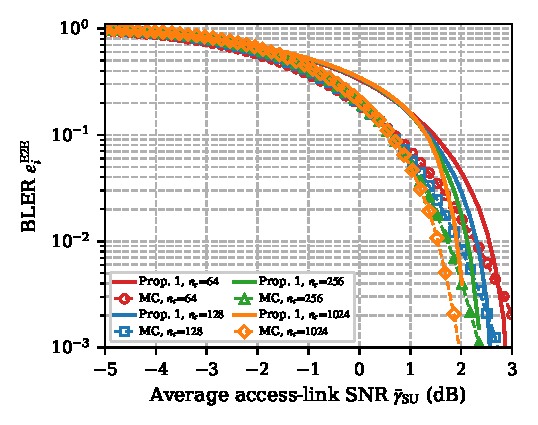
\includegraphics[width=\columnwidth]{prop1_closedform_validation.eps}
  \caption{Subchannel BLER versus average access-link SNR for different per-subchannel blocklengths $n_c$ under dominant-LOS Rician fading: simulation and closed-form
  approximation in Proposition~\ref{prop:bler_approx}. Feeder-link sensitivity is shown for $n_c = 256$ with $\bar{\gamma}_{i,\mathrm{GS}}/\bar{\gamma}_{i,\mathrm{SU}} = 10$~dB and $3$~dB.}
    \label{fig:prop1_validation}
\end{figure}

Fig.~\ref{fig:prop2_diversity} verifies Proposition~\ref{prop:bler_high_snr} and Corollary~\ref{cor:bler_rayleigh} by plotting the subchannel BLER under pure Rayleigh fading for different DD diversity orders $L$. Three curve families are shown: the closed-form expression from Corollary~\ref{cor:bler_rayleigh}, the high-SNR asymptotic form from Proposition~\ref{prop:bler_high_snr}, and simulation. At moderate-to-high SNR, the asymptotic and closed-form curves converge and both match the simulation results closely, confirming that the analytical framework accurately captures the diversity behaviour of the multipath channel model in~\eqref{eq:combined_snr_final}. At low SNR, the high-SNR asymptotic form deviates from the simulation and closed-form results because the leading-term approximation of the regularised incomplete gamma function requires $\hat{\gamma}_{i,\mathrm{NLOS}} \gg \psi_i$, a condition that is not satisfied in the low-SNR regime. 



\begin{figure}[t]
    \centering
    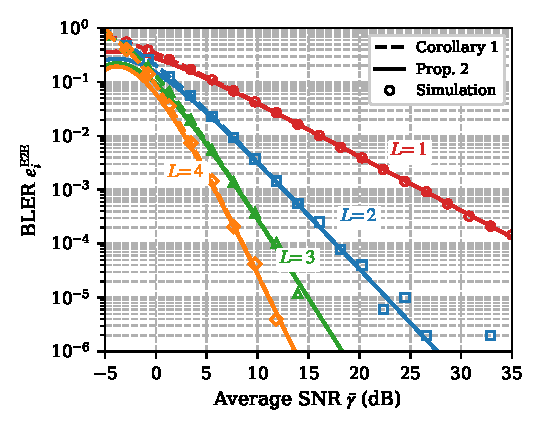
\includegraphics[width=\columnwidth]{prop2_diversity_order.eps}
  \caption{Subchannel BLER versus average access-link SNR for different DD diversity orders under Rayleigh fading: simulation, closed-form
  in Corollary~\ref{cor:bler_rayleigh}, and high-SNR asymptotic in Proposition~\ref{prop:bler_high_snr}.}
  \label{fig:prop2_diversity}
\end{figure}

Fig.~\ref{fig:bler_vs_power} presents BLER versus total
transmit power $P_{\mathrm{total}}$. As power increases, the
diversity transform scheme achieves a more rapid BLER reduction than the standard polar code configurations, consistently outperforming both interleaved and non-interleaved baselines across the entire power
range. The gap between the two increases at higher power levels, where
the diversity transform can exploit the improved subchannel quality
more effectively. The PPV bounds from Theorem~\ref{thm:fbl_bler}
track the simulation results with a consistent offset attributable
to the suboptimality of the practical SCL decoder relative to the
channel capacity. Notably, the PPV bound with diversity is substantially lower than its counterpart without diversity, highlighting the theoretical advantage of the diversity transform. 

\begin{figure}[t]
    \centering
    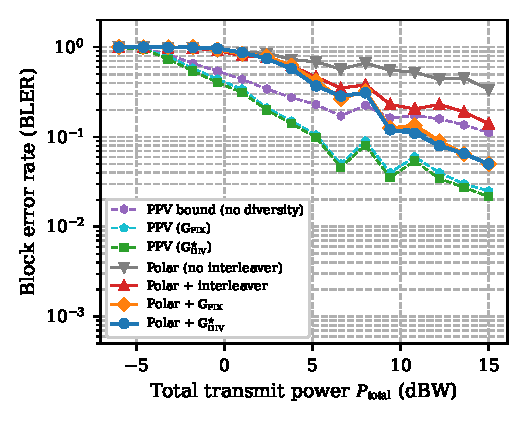
\includegraphics[width=\columnwidth]{bler_comparison.eps}
    \caption{System BLER versus total transmit power $P_{\mathrm{total}}$ at
    reference elevation $\epsilon = 40^{\circ}$.}
    \label{fig:bler_vs_power}
\end{figure}


Fig.~\ref{fig:bler_vs_elevation} evaluates elevation-angle sensitivity.
At low elevation, all evaluated schemes saturate near unity BLER due to high path
loss, increased atmospheric attenuation, and severe blockage
probability. As the elevation angle increases, the propagation
conditions improve and the blockage probability decreases, allowing
more subchannels to contribute reliably to the MDS recovery guaranteed by Theorem~\ref{thm:block_mds}. The diversity advantage increases correspondingly: at zenith, the diversity transform scheme reduces the BLER by approximately 50\% relative to the non-interleaved polar code, while the PPV bound with diversity drops by more than 90\% relative to the bound without diversity.

\begin{figure}[t]
    \centering
    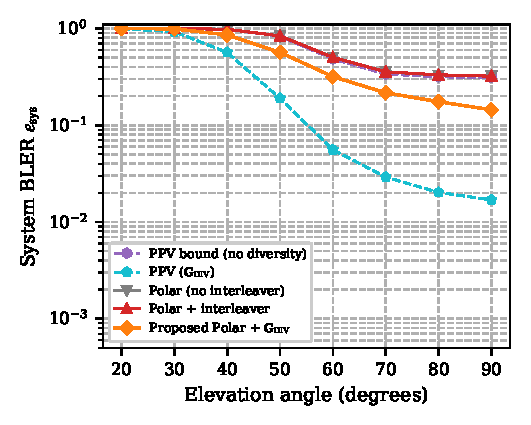
\includegraphics[width=\columnwidth]{bler_vs_elevation_comparison.eps}
    \caption{System BLER versus elevation angle $\epsilon$ at $P_{\mathrm{total}} = 8$~dBW with $n_{\mathrm{s}} = 6$ subchannels and $(N,K) = (256,128)$ polar code.}
    \label{fig:bler_vs_elevation}
\end{figure}

Fig.~\ref{fig:bler_vs_blocklength} examines how the system BLER varies with the codeword blocklength $N$ at a fixed rate $R_c = 0.5$. The BLER decreases with $N$ for all schemes, as longer codes provide greater error‑correction capability. The diversity transform maintains a consistent advantage across all blocklengths, with the largest relative gain at short blocklengths, where the standalone polar code is most susceptible to deep fades on individual subchannels. As $N$ increases, the performance gap narrows because the stronger polar code can independently recover from moderate fading without the diversity layer.  Notably, bit interleaving within
  each subchannel provides negligible gain over the non-interleaved baseline, confirming that the dominant impairment is inter-subchannel blockage rather than
  intra-subchannel fading.

\begin{figure}[t]
    \centering
    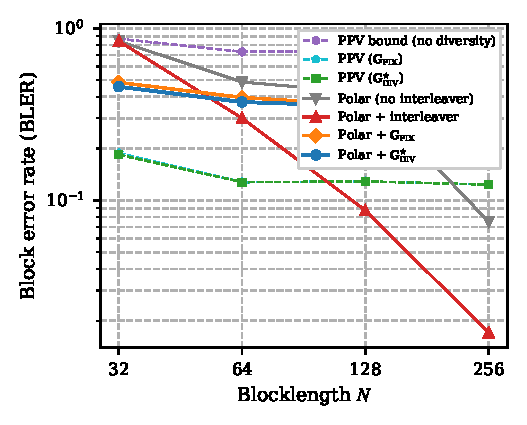
\includegraphics[width=\columnwidth]{bler_vs_blocklength.eps}
    \caption{System BLER versus polar code blocklength $N$ at 
    $P_{\mathrm{total}} = 10$~dBW.}
    \label{fig:bler_vs_blocklength}
\end{figure}

Fig.~\ref{fig:bler_vs_blockage} plots the system BLER versus the per-subchannel blockage probability. At low blockage, all schemes achieve comparable BLER, with the diversity transform introducing only a modest overhead due to its reduced effective code rate. As blockage increases, the standalone polar code configurations, both with and without interleaving, rise rapidly toward unity BLER because a single blocked subchannel leads to unrecoverable data loss. In contrast, the diversity-transform-based scheme degrades gracefully, maintaining a significantly lower BLER throughout the blockage range. This robustness follows directly from Theorem~\ref{thm:block_mds}: the MDS structure guarantees full data recovery whenever at least $k_{\mathrm{c}}$ of the $n_{\mathrm{s}}$ subchannels survive. Even at the highest blockage probability considered, the diversity transform outperforms all baselines by a wide margin, confirming that the erasure protection provided by the MDS code more than compensates for the rate overhead.
\begin{figure}[t]
    \centering
    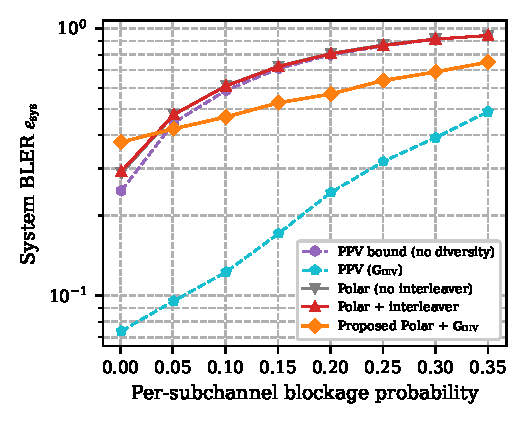
\includegraphics[width=\columnwidth]{bler_vs_blockage.eps}
    \caption{System BLER versus per-subchannel blockage probability at $P_{\mathrm{total}} = 8$~dBW with $n_{\mathrm{s}} = 6$ subchannels and $d_{\min} = 3$.}
    \label{fig:bler_vs_blockage}
\end{figure}

Fig.~\ref{fig:bler_correlated_blockage} evaluates the system
BLER as a function of the blockage correlation parameter
$\rho_{\mathrm{blk}}$ using the Gaussian copula model
in~\eqref{eq:corr_matrix_blk}, with a fixed per-subchannel blockage probability of $0.2$.
At $\rho_{\mathrm{blk}} = 0$, the diversity transform achieves substantially lower BLER than the baselines, consistent with the
independent-blockage results in Fig.~\ref{fig:bler_vs_blockage}.
As $\rho_{\mathrm{blk}}$ increases, the gap narrows because correlated blockage drives the failure
distribution toward two extremes: either all subchannels survive or all are simultaneously blocked. In the former case, the diversity transform
is unnecessary, whereas in the latter, no scheme can recover the data once
more than $f_{\max}$ subchannels are lost.
Consequently, the partial-failure regime, where the MDS recovery
guarantee of Theorem~\ref{thm:block_mds} is most effective, becomes less probable under strong correlation.
For moderate correlation
($\rho_{\mathrm{blk}} \leq 0.8$), the diversity transform
consistently achieves the lowest BLER.
Beyond $\rho_{\mathrm{blk}} \approx 0.85$, however, the baselines
outperform the diversity transform. In this regime, blockage events become nearly common across all subchannels, reducing the benefit of algebraic erasure protection. Consequently, the rate overhead of the MDS diversity
code ($\varrho/n_{\mathrm{out}} = 2/3$) outweighs its recovery gain.
This crossover indicates that the diversity transform is most
effective in the low-to-moderate correlation regime relevant to LEO NTN systems with spatially
separated satellites.  Accordingly, the diversity transform can be adaptively disabled when
the predicted correlation becomes very high.
In practice, co-visible LEO satellites at different orbital positions are subject to moderate blockage,
resulting in partial subchannel failures that are well suited to
algebraic erasure recovery.

\begin{figure}[t]
    \centering
    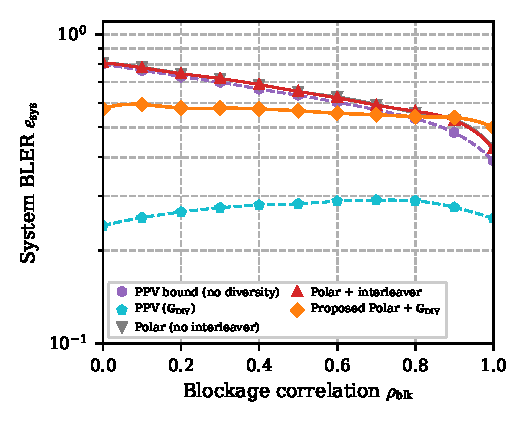
\includegraphics[width=\columnwidth]{bler_vs_correlated_blockage.eps}
    \caption{System BLER versus blockage correlation
    $\rho_{\mathrm{blk}}$ at per-subchannel blockage probability $0.2$.}
    \label{fig:bler_correlated_blockage}
\end{figure}

Fig.~\ref{fig:bler_vs_nsubchannels} examines how BLER scales with the
number of subchannels $n_{\mathrm{s}}$, where
$k_{\mathrm{c}} = \max(n_{\mathrm{s}} - 2, 1)$ maintains a fixed
erasure tolerance of $d_{\min} - 1 = 2$. For the minimal configuration ($n_{\mathrm{s}}=2$), all schemes exhibit high BLER, as the number of available subchannels is too small to provide sufficient diversity. The diversity advantage increases with $n_{\mathrm{s}}$: at the largest configuration tested, the diversity transform scheme reduces the BLER by approximately 80\% relative to the non-interleaved polar code, consistent with the scaling predicted by Corollary~\ref{cor:sys_bler_poisson}. This improvement arises
because increasing $n_{\mathrm{s}}$ at fixed $d_{\min}$ enlarges the
family of recoverable erasure patterns in Theorem~\ref{thm:block_mds},
providing more spatial diversity paths through the multi-satellite
constellation.

\begin{figure}[t]
    \centering
    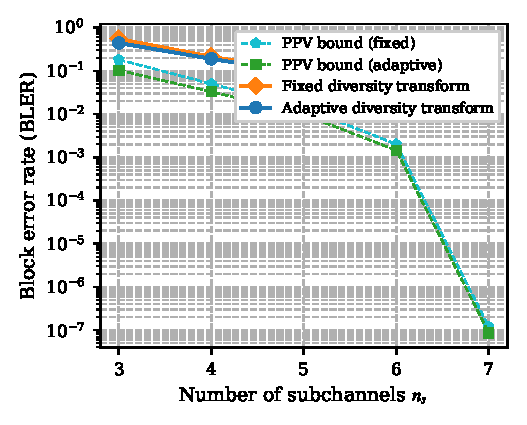
\includegraphics[width=\columnwidth]{bler_vs_n_subchannels.eps}
    \caption{System BLER versus number of subchannels $n_{\mathrm{s}}$ with
    $k_{\mathrm{c}} = \max(n_{\mathrm{s}} - 2, 1)$ at
    $P_{\mathrm{total}} = 3$~dBW.}
    \label{fig:bler_vs_nsubchannels}
\end{figure}

Fig.~\ref{fig:otfs_vs_ofdm} compares the BLER performance of OTFS- and OFDM-based schemes as a function of the normalized Doppler shift $f_D / \Delta f$. OTFS-based schemes maintain nearly constant BLER across the evaluated range.  In contrast, OFDM-based schemes exhibit increased BLER at higher normalized Doppler values due to inter-carrier interference (ICI). At the highest normalized Doppler shift tested, the BLER of the OFDM scheme with diversity transform is significantly higher than that of the corresponding OTFS scheme. At zero Doppler, the two waveforms perform comparably since ICI is absent; however, this equivalence disappears rapidly as Doppler increases and the OFDM subcarrier orthogonality is lost. The OTFS baselines without diversity also
remain stable, whereas the corresponding OFDM baselines degrade
noticeably. In addition, the standalone polar code curves with and without interleaving overlap because interleaving only permutes bits within a single subchannel and therefore cannot recover information lost when an entire subchannel is blocked. These results confirm that DD domain processing with OTFS, combined with the proposed diversity transform, is well suited to the high Doppler shifts characteristic of LEO satellite links.
To quantify the impact of fractional Doppler and imperfect
channel estimation, Fig.~\ref{fig:otfs_vs_ofdm} also includes the
proposed OTFS scheme under two additional impairment conditions:
(i)~fractional Doppler with worst-case offset $\alpha_p = 0.5$ and perfect channel estimation; and
(ii)~fractional Doppler combined with imperfect channel estimation
($\sigma_{\mathrm{CSI}}^2 = 0.01$, corresponding to a channel estimation MSE of $-20$~dB, which is representative of embedded pilot-aided OTFS estimation at moderate SNR~\cite{Raviteja2018}).
Both impaired OTFS curves exhibit a moderate BLER increase (approximately
$1.5$--$2$ times) relative to the ideal integer-Doppler case, yet
remain significantly below the OFDM curves at high normalised Doppler.
This confirms that the OTFS advantage over OFDM is preserved under
realistic impairments, and that the diversity transform's
subchannel-level recovery guarantee of Theorem~\ref{thm:block_mds}
remains effective.
\begin{figure}[t]
    \centering
    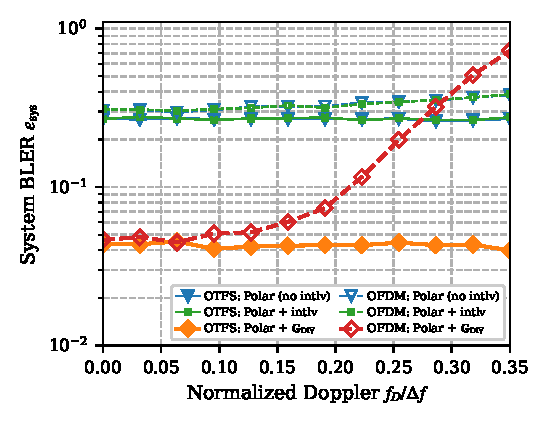
\includegraphics[width=\columnwidth]{otfs_vs_ofdm.eps}
    \caption{BLER versus normalised Doppler $f_{D}/\Delta f$ for OTFS
     and OFDM at $P_{\mathrm{total}} = 20$~dBW, including fractional
     Doppler and imperfect channel estimation impairments.}
    \label{fig:otfs_vs_ofdm}
\end{figure}

Fig.~\ref{fig:throughput} presents the effective throughput as a function of total transmit power $P_{\mathrm{total}}$ for six schemes. The per-subchannel polar baselines (with and without interleaving) transmit independent data on each subchannel at effective rate $\eta_{\mathrm{eff}} = R_c (1 - \epsilon_{\mathrm{sys}})$, where $R_c = 0.5$. The diversity transform accounts for the MDS rate overhead $\varrho/n_{\mathrm{out}} = 12/18 = 2/3$, yielding $\eta_{\mathrm{eff}} = R_c \cdot (\varrho / n_{\mathrm{out}}) \cdot (1 - \epsilon_{\mathrm{sys}}) \approx 0.33 \cdot (1 - \epsilon_{\mathrm{sys}})$. Rate-optimised MRC and SC are also included. Both schemes repeat the same codeword on all $n_{\mathrm{s}}$ subchannels, giving throughput $\eta_{\mathrm{MRC/SC}} = (R/n_{\mathrm{s}}) \cdot (1 - \epsilon)$, where $R$ is optimised at each operating point to maximise throughput given the combined SNR ($\gamma_{\mathrm{MRC}} = \sum_j \gamma_j$ for MRC, $\gamma_{\mathrm{SC}} = \max_j \gamma_j$ for SC). Despite adaptive rate optimisation, MRC and SC saturate at approximately $0.16$~bits per channel use because of the $1/n_{\mathrm{s}}$ repetition penalty.
Although the diversity transform operates at a lower effective rate than the per-subchannel polar baselines, it achieves higher throughput in the medium-power regime ($6$--$20$~dBW), where the substantial reduction in $\epsilon_{\mathrm{sys}}$ outweighs the MDS rate overhead. The diversity transform surpasses rate-optimised MRC at $P_{\mathrm{total}} \approx 12$~dBW and achieves nearly twice the MRC throughput at $25$~dBW. At high power ($P_{\mathrm{total}} > 22$~dBW), the $\epsilon_{\mathrm{sys}}$ of the per-subchannel polar baselines decreases sufficiently for their higher effective rate ($R_c = 0.5$) to dominate, and their throughput converges with that of the diversity transform. This transition aligns with the design objective: the diversity transform is designed for the power-limited LEO NTN operating regime, where blockage and fading are the dominant impairments. This corresponds to the conditions under which Theorem~\ref{thm:block_mds} provides the greatest erasure recovery benefit.

\begin{figure}[t]
    \centering
    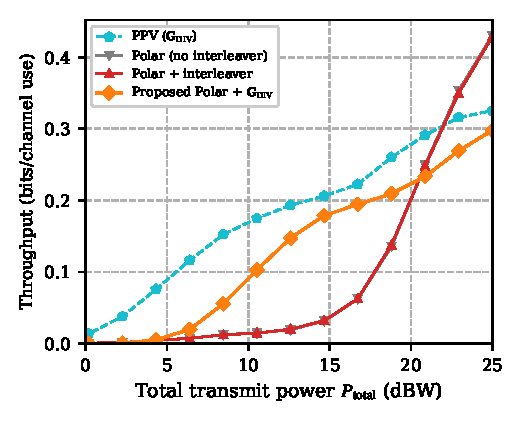
\includegraphics[width=\columnwidth]{throughput_reliability.eps}
    \caption{Effective throughput versus
   total transmit power at $\epsilon = 40^{\circ}$ with $n_{\mathrm{s}} = 6$ subchannels. The diversity transform operates at effective rate $R_c \cdot \varrho/n_{\mathrm{out}} \approx 0.33$; per-subchannel baselines at $R_c = 0.5$. MRC and SC are rate-optimised at each power level.}
    \label{fig:throughput}
\end{figure}

 Fig.~\ref{fig:latency_comparison} demonstrates the latency advantage
of the diversity transform over MRC, SC, and the HARQ-CC baseline
in~\eqref{eq:harq_bler}--\eqref{eq:harq_latency},
configured with $K_{\max} = 4$,
$T_{\mathrm{RTT}} = 20$~ms~\cite{3GPP38821}, and persistent
blockage across retransmission attempts.
Latency values are geometric means over channel realisations.
MRC combines LLRs from all non-blocked subchannels (effective SNR $= \sum_j \bar{\gamma}_j$), and SC selects the subchannel with the highest instantaneous SNR; both repeat the same codeword on every subchannel and therefore require $k_c$ times more channel uses to deliver the same message size.
Despite
the chase combining advantage, the diversity transform consistently achieves
lower transmission latency than all three baselines across all operating points.
For example, at $P_{\mathrm{total}} = 10$~dBW and $\epsilon_{\mathrm{sys}}^{\mathrm{target}} = 10^{-3}$, the diversity transform achieves approximately three times lower latency than HARQ-CC.
As the target system BLER $\epsilon_{\mathrm{sys}}^{\mathrm{target}}$
becomes stricter, HARQ-CC latency grows faster because each
additional retransmission round adds a full round-trip time, while MRC and SC latency grows because their per-subchannel codeword must be $k_c$ times longer to deliver the same message. This latency
reduction follows directly from the single-shot decoding guarantee of
Corollary~\ref{cor:latency_reduction}: the MDS structure of
$\mathbf{G}_{\mathrm{DIV}}$ relaxes the per-subchannel BLER target
to $\epsilon^{*} \gg \epsilon_{\mathrm{sys}}^{\mathrm{target}}$,
enabling a shorter blocklength without feedback-driven retransmissions
by exploiting spatial diversity across co-visible satellites within a
single OTFS frame.

\begin{figure}[t]
    \centering
    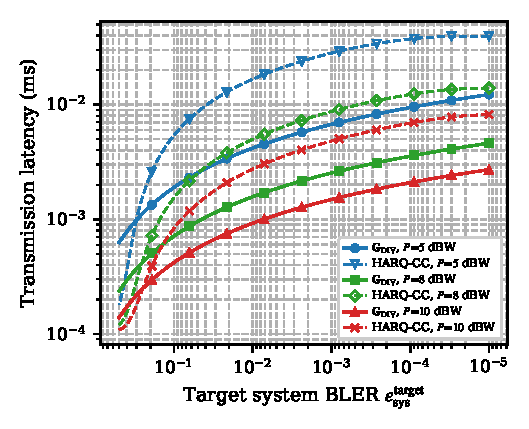
\includegraphics[width=\columnwidth]{latency_comparison.eps}
  \caption{Transmission latency versus target system BLER $\epsilon_{\mathrm{sys}}^{\mathrm{target}}$ for the diversity transform, MRC, SC, and HARQ-CC ($K_{\max} = 4$, $T_{\mathrm{RTT}} = 20$~ms) at $P_{\mathrm{total}} = 5$ and $10$~dBW. MRC and SC require $k_c = 4$ times more channel uses to deliver the same message size.}
    \label{fig:latency_comparison}
\end{figure}

Fig.~\ref{fig:bler_robustness} evaluates the robustness of the
proposed diversity transform under imperfect subchannel reliability prediction, as
characterised by Proposition~\ref{prop:bler_imperfect}.
The prediction-error standard deviation $\sigma_p$ is
swept from $0$~dB (perfect prediction) to $4$~dB, spanning
the range of realistic mismatch from ephemeris error, UE
location uncertainty, and atmospheric model deviation.
The system BLER degrades gracefully with increasing $\sigma_p$:
at $P_{\mathrm{total}} = 25$~dBW, the BLER increases from
$0.105$ at $\sigma_p = 0$~dB to $0.139$ at $\sigma_p = 4$~dB,
a modest absolute BLER increase of $0.034$.
All diversity transform curves remain significantly
below the polar (no diversity) baseline across the operating
range, confirming that the MDS redundancy effectively mitigates the increased per-subchannel failure rate from prediction mismatch. The system BLER in~\eqref{eq:sys_bler_imperfect} decays proportionally to $(\check{\epsilon}_i^{\mathrm{E2E}})^{d_{\min}}$, preserving the MDS diversity order $d_{\min}$ regardless of
  $\sigma_p$.

\begin{figure}[t]
    \centering
    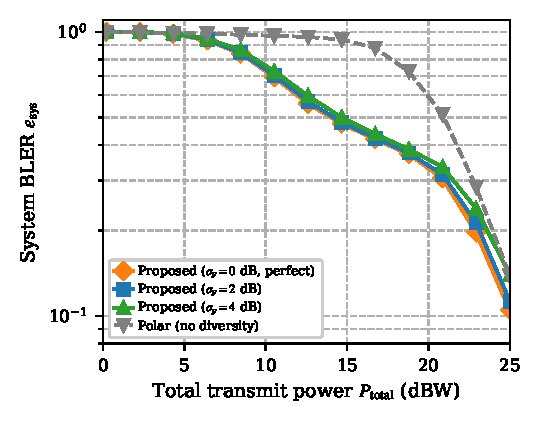
\includegraphics[width=\columnwidth]{bler_robustness_prediction.eps}
    \caption{System BLER versus total transmit power under imperfect
    prediction with combined prediction error $\sigma_p$.}
    \label{fig:bler_robustness}
\end{figure}

Fig.~\ref{fig:latency_robustness} shows the corresponding latency
impact of prediction imperfections on transmission at $P_{\mathrm{total}} = 10$~dBW.
The diversity transform with $\sigma_p = 0$--$4$~dB consistently
achieves lower latency than HARQ-CC across all target system BLER
values, confirming that the latency reduction predicted by~\eqref{eq:min_blocklength_imperfect} is preserved under
realistic prediction imperfections.
At $\sigma_p = 4$~dB, the latency penalty relative to perfect
prediction remains modest, with less than a twofold increase at
$\epsilon_{\mathrm{sys}}^{\mathrm{target}} = 10^{-4}$, while
still achieving approximately two times lower latency than
HARQ-CC.
These results demonstrate that the single-shot decoding advantage
enabled by the diversity transform remains robust to prediction mismatch.

\begin{figure}[t]
    \centering
    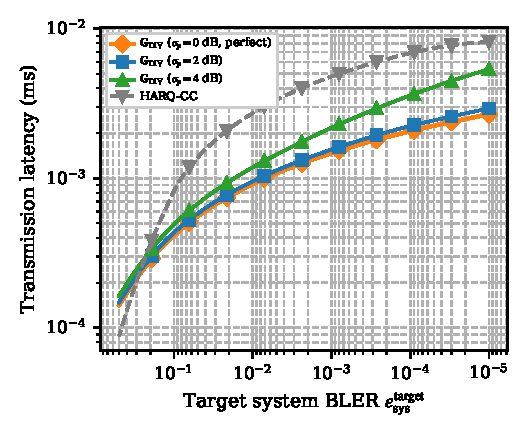
\includegraphics[width=\columnwidth]{latency_robustness_prediction.eps}
    \caption{Transmission latency versus target system BLER under
    imperfect prediction at $P_{\mathrm{total}} = 10$~dBW.}
    \label{fig:latency_robustness}
\end{figure}

Fig.~\ref{fig:bler_vs_threshold} examines the sensitivity
of the system BLER to the erasure threshold
$\epsilon_{\mathrm{th}}$.
The MDS recovery guarantee of Theorem~\ref{thm:block_mds} is
independent of this threshold; however, the choice of
$\epsilon_{\mathrm{th}}$ affects the trade-off between
unnecessary erasure declarations (low $\epsilon_{\mathrm{th}}$,
increasing MDS redundancy consumption) and undetected FEC failures
(high $\epsilon_{\mathrm{th}}$, admitting degraded subchannels).
At $P_{\mathrm{total}} = 25$~dBW, the system BLER exhibits a
clear minimum near $\epsilon_{\mathrm{th}} = 0.05$--$0.1$ and
rises on both sides, confirming this trade-off.
At lower power levels, the system BLER is broadly insensitive
to $\epsilon_{\mathrm{th}}$ over more than two orders of magnitude.
The value $\epsilon_{\mathrm{th}} = 0.1$ adopted throughout this
paper lies within the near-optimal region across all evaluated
power levels.

\begin{figure}[t]
    \centering
    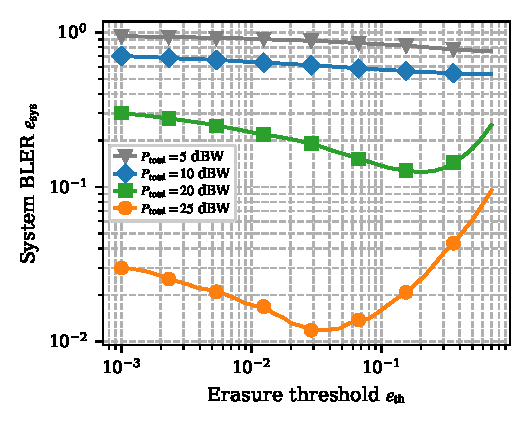
\includegraphics[width=\columnwidth]{bler_vs_threshold.eps}
    \caption{System BLER versus erasure threshold
    $\epsilon_{\mathrm{th}}$ at different transmit power levels.}
    \label{fig:bler_vs_threshold}
\end{figure}

Fig.~\ref{fig:fec_comparison} demonstrates the FEC-agnostic operation of the proposed diversity transform by comparing polar codes (SCL decoding, list size~$32$) and LDPC codes (BP decoding, $50$ iterations) at three code rates $R_c \approx 1/4$, $1/2$, and $3/4$. All codes are combined with the diversity transform $\mathbf{G}_{\mathrm{DIV}}$ and evaluated under identical channel conditions. At each code rate, the polar and LDPC curves are nearly indistinguishable, with the residual gap remaining below $0.2$~dB across the entire power range. This confirms that the system BLER is dominated by the diversity transform's erasure recovery mechanism rather than by the specific FEC decoder, confirming FEC-agnostic operation. The diversity gain is largest at higher code rates: at $R_c = 3/4$, the no-diversity baseline remains above $0.25$ even at $P_{\mathrm{total}} = 23$~dBW, whereas the diversity-transform-equipped schemes reach $0.03$, because the weaker FEC protection makes the system more reliant on the erasure recovery provided by $\mathbf{G}_{\mathrm{DIV}}$. At $R_c = 1/4$, the stronger FEC narrows the gap, but the diversity transform still provides a consistent advantage across all power levels.

\begin{figure}[t]
    \centering
    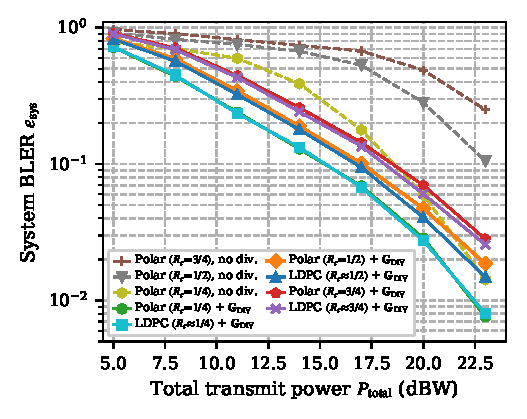
\includegraphics[width=\columnwidth]{fec_comparison.eps}
    \caption{System BLER versus total transmit power for polar and LDPC codes with the proposed diversity transform. No-diversity baselines shown for reference.}
    \label{fig:fec_comparison}
\end{figure}


In summary, the simulation results show that the diversity transform yields lower BLER than conventional standalone FEC and FEC with interleaving across the evaluated parameters, including transmit power, elevation angle, polar code blocklength, per-subchannel blockage probability, and number of subchannels. The reduction in BLER is greater under conditions where individual subchannels are more likely to experience outage, specifically at high blockage probability (Fig.~\ref{fig:bler_vs_blockage}) and when the number of available subchannels is large (Fig.~\ref{fig:bler_vs_nsubchannels}). This behavior is consistent with the MDS erasure correction capability described in Theorem~\ref{thm:block_mds}, which becomes more effective as the number of recoverable erasure patterns increases. The combination of OTFS and the diversity transform maintains stable performance under high Doppler shifts where OFDM degrades significantly (Fig.~\ref{fig:otfs_vs_ofdm}). The FEC comparison in Fig.~\ref{fig:fec_comparison} confirms that the diversity transform operates independently of the underlying FEC scheme: polar and LDPC codes achieve nearly identical BLER at all code rates when combined with $\mathbf{G}_{\mathrm{DIV}}$, indicating that the system performance is governed by the erasure recovery capability rather than the specific decoder. Finally, single-shot decoding eliminates the round‑trip latency associated with HARQ retransmissions and achieves lower latency than MRC and SC baselines when normalised for equal message size (Fig.~\ref{fig:latency_comparison}), consistent with the latency reduction established in Corollary~\ref{cor:latency_reduction}. This indicates that spatial diversity across co‑visible LEO satellites can replace temporal diversity via retransmissions.

\vspace{-.5cm}
\section{Conclusion}
\label{sec:conclusion}
This paper presented a diversity transform framework for OTFS-based LEO NTN downlinks that enables deterministic recovery from simultaneous satellite outages without retransmissions. The proposed approach significantly reduces the system BLER compared to standalone polar-coded baselines under low elevation angles and severe blockage conditions, while outperforming MRC, SC, and HARQ-CC in both latency and throughput. The modular architecture is FEC-agnostic and supports single-shot decoding, eliminating HARQ round-trip latency and achieving more than 70\% reduction in median transmission latency under strict reliability targets. Theoretical analysis established guaranteed full-rank recovery from subchannel erasures, while finite-blocklength BLER and latency analyses were validated through extensive simulations under realistic LEO NTN conditions. Overall, the results demonstrate that spatial diversity across co-visible LEO satellites can effectively replace retransmission-based temporal diversity, enabling reliable and low-latency SatCom resilient to correlated outages, Doppler effects, and prediction imperfections without requiring CSI feedback or retransmissions.
\begin{comment}
This paper presents a diversity transform layer for LEO NTN downlinks  that enables deterministic recovery from erasures under simultaneous satellite  outages without requiring retransmissions. The results demonstrate that the proposed approach reduces the system block error rate by a wide margin compared to standalone polar coding baselines, both with and without interleaving, at low elevation angles and under high blockage conditions. The diversity transform also outperforms MRC, SC, and HARQ-CC across latency and throughput metrics, overcoming the fundamental spectral efficiency ceiling of repetition-based combining. The modular architecture is FEC-agnostic, enabling composition with any coding scheme without cross-layer redesign. In addition, the single-shot decoding property eliminates the round-trip latency penalty associated with HARQ, resulting in more than 70\% reduction in median transmission latency for strict reliability targets, and the system remains robust to prediction imperfections.
The central theoretical contribution establishes that 
a binary diversity 
transform derived from an MDS code guarantees full-rank recovery 
whenever the number of surviving subchannels is at least the code 
dimension. 
The proposed finite-blocklength BLER framework and latency analysis are further validated through extensive simulation results, confirming the reliability and low-latency advantages of the proposed architecture under realistic LEO NTN conditions. 
Collectively, these results demonstrate that the proposed framework enables reliable and low-latency SatCom without requiring CSI feedback or retransmissions, while outperforming conventional baselines. The primary practical implication is that spatial diversity across co‑visible LEO satellites can replace retransmission‑based temporal diversity, enabling single‑shot recovery from erasures. By relaxing the per-subchannel BLER requirement, the proposed architecture enables a single OTFS frame to meet the target system reliability while remaining resilient to correlated outages and high Doppler shifts.
\end{comment}

%======================================================================
%======================================================================
\appendices

\section{Proof of Theorem~\ref{thm:fbl_bler}}
\label{app:proof_fbl_bler}
From~\cite{Polyanskiy2010}, setting $R^*(n_c,\epsilon,\gamma)=R_c$ in~\eqref{eq:normal_approx} and inverting with respect to $\epsilon$ gives the conditional BLER at instantaneous SNR $\gamma$:
\begin{equation}
\epsilon(\gamma)=Q\!\left(\frac{\sqrt{n_c}\bigl(C(\gamma)-R_c\bigr)+\frac{\log_2 n_c}{2\sqrt{n_c}}}{\sqrt{V(\gamma)}}\right).
\label{eq:cond_proof}
\end{equation}
In the regime $\bar{\gamma}_{i,\mathrm{GS}}\gg\gamma_{i,\mathrm{SU}}^{\mathrm{MRC}}$, substituting~\eqref{eq:feeder_deterministic} into~\eqref{eq:combined_snr_full} gives
\begin{equation}
\gamma_i^{\mathrm{c}}\approx\gamma_{i,\mathrm{SU}}^{\mathrm{MRC}}=\bar{\gamma}_{i,\mathrm{SU}}\sum_{p=0}^{L_i-1}P_{i,\mathrm{SU},p}\,|g_{i,\mathrm{SU},p}|^2.
\label{eq:snr_step1}
\end{equation}
Applying the dominant-LOS approximation $K_{i,\mathrm{SU},0}\!\gg\!1$ and $K_{i,\mathrm{SU},p}\!=\!0$ for $p\!\geq\!1$, \eqref{eq:snr_step1} can be expressed as
\begin{equation}
\gamma_i^{\mathrm{c}}=\underbrace{\bar{\gamma}_{i,\mathrm{SU}}P_{i,\mathrm{SU},0}}_{=\,\gamma_{i,0}^{\mathrm{det}}}+\underbrace{\bar{\gamma}_{i,\mathrm{SU}}\sum_{p=1}^{L_i-1}P_{i,\mathrm{SU},p}\,|g_{i,\mathrm{SU},p}|^2}_{=\,\gamma_i^{\mathrm{NLOS}}}.
\label{eq:snr_decomp}
\end{equation}
Since $|g_{i,\mathrm{SU},p}|^2\overset{\mathrm{i.i.d.}}{\sim}\mathrm{Exp}(1)$ for $p\geq1$, it follows that
\begin{equation}
\gamma_i^{\mathrm{NLOS}}\sim\mathrm{Gamma}\!\left(L_i-1,\,\hat{\gamma}_{i,\mathrm{NLOS}}\right),\quad\hat{\gamma}_{i,\mathrm{NLOS}}=\frac{\bar{\gamma}_{i,\mathrm{SU}}P_{\mathrm{NLOS}}}{L_i-1}.
\label{eq:nlos_dist}
\end{equation}
From~\eqref{eq:snr_decomp} and~\eqref{eq:nlos_dist}, the CDF of $\gamma_i^{\mathrm{c}}$ is
\begin{IEEEeqnarray}{rCl}
F_{\gamma_i^{\mathrm{c}}}(\gamma)&=&\Pr\!\left(\gamma_i^{\mathrm{NLOS}}\leq\gamma-\gamma_{i,0}^{\mathrm{det}}\right)\nonumber\\
&=&\Upsilon\!\left(L_i-1,\,\frac{\gamma-\gamma_{i,0}^{\mathrm{det}}}{\hat{\gamma}_{i,\mathrm{NLOS}}}\right),\quad\gamma\geq\gamma_{i,0}^{\mathrm{det}},
\label{eq:cdf_step}
\end{IEEEeqnarray}
which coincides with~\eqref{eq:combined_cdf}. Since the channel is quasi-static over each OTFS frame, averaging \eqref{eq:cond_proof} over the distribution of $\gamma_i^{\mathrm{c}}$ gives
\begin{IEEEeqnarray}{rCl}
\epsilon_i^{\mathrm{E2E}}&=&\mathbb{E}_{\gamma_i^{\mathrm{c}}}\!\left[\epsilon(\gamma_i^{\mathrm{c}})\right]\nonumber\\
&=&\int_{\gamma_{i,0}^{\mathrm{det}}}^{\infty}Q\!\left(\frac{\sqrt{n_c}\bigl(C(\gamma)-R_c\bigr)+\frac{\log_2 n_c}{2\sqrt{n_c}}}{\sqrt{V(\gamma)}}\right)f_{\gamma_i^{\mathrm{c}}}(\gamma)\,d\gamma,
\nonumber
\end{IEEEeqnarray}
where the lower limit follows from $F_{\gamma_i^{\mathrm{c}}}(\gamma)=0$ for $\gamma<\gamma_{i,0}^{\mathrm{det}}$. This is~\eqref{eq:bler_exact}, completing the proof.

\section{Proof of Proposition~\ref{prop:bler_approx}}
\label{app:proof_bler_approx}
Substituting the piecewise approximation~\eqref{eq:piecewise_approx} into~\eqref{eq:bler_exact} and exchanging the order of integration following~\cite{Makki2014} gives
\begin{IEEEeqnarray}{rCl}
\epsilon_i^{\mathrm{E2E}}&\approx&\int_{\phi_i}^{\delta_i}\!\left(\tfrac{1}{2}-\beta_i\sqrt{n_c}(\gamma_i-\psi_i)\right)f_{\gamma_i^{\mathrm{c}}}(\gamma_i)\,d\gamma_i\nonumber\\
&+&F_{\gamma_i^{\mathrm{c}}}(\phi_i)\nonumber\\
&=&\beta_i\sqrt{n_c}\int_{\phi_i}^{\delta_i}F_{\gamma_i^{\mathrm{c}}}(\gamma_i)\,d\gamma_i.
\label{eq:bler_approx_integral}
\end{IEEEeqnarray}
Since $\delta_i-\phi_i=({\beta_i\sqrt{n_c}})^{-1}\to0$ as $n_c\to\infty$, the mean value theorem applied to~\eqref{eq:bler_approx_integral} gives \cite{Makki2014,Basnayaka2022}
\begin{equation}
\epsilon_i^{\mathrm{E2E}}\approx\beta_i\sqrt{n_c}\cdot F_{\gamma_i^{\mathrm{c}}}(\psi_i)\cdot(\delta_i-\phi_i)=F_{\gamma_i^{\mathrm{c}}}(\psi_i).
\label{eq:bler_cdf_step}
\end{equation}
Substituting the CDF from~\eqref{eq:cdf_step} into~\eqref{eq:bler_cdf_step} gives~\eqref{eq:bler_cdf_combined}.

\section{Proof of Proposition~\ref{prop:bler_high_snr}}
\label{app:proof_bler_high_snr}
The regularised incomplete gamma function in~\eqref{eq:bler_cdf_combined} admits the series expansion
\begin{equation}
\Upsilon(a,x)=\frac{x^a e^{-x}}{\Gamma(a)}\sum_{k=0}^{\infty}\frac{x^k}{\prod_{j=0}^{k}(a+j)}.
\label{eq:gamma_series}
\end{equation}
For $x\ll a$, the $k=0$ term dominates in~\eqref{eq:gamma_series}, giving
\begin{equation}
\Upsilon(a,x)\approx\frac{x^a e^{-x}}{a\,\Gamma(a)}=\frac{x^a e^{-x}}{\Gamma(a+1)}.
\label{eq:gamma_approx}
\end{equation}
Setting $a=L_i-1$ and $x=\xi_i\triangleq(\psi_i-\gamma_{i,0}^{\mathrm{det}})/\hat{\gamma}_{i,\mathrm{NLOS}}$ in~\eqref{eq:gamma_approx}, and noting that $\Gamma(L_i)=(L_i-1)!$, gives
\begin{equation}
\epsilon_i^{\mathrm{E2E}}\approx\frac{\xi_i^{L_i-1}\,e^{-\xi_i}}{(L_i-1)!},
\end{equation}
which is~\eqref{eq:bler_high_snr}. The condition $x\ll a$ is equivalent to $\xi_i\ll L_i-1$, satisfied in the high-SNR regime where $\hat{\gamma}_{i,\mathrm{NLOS}}\gg\psi_i-\gamma_{i,0}^{\mathrm{det}}$.

\section{Proof of Corollary~\ref{cor:bler_rayleigh}}
\label{app:proof_bler_rayleigh}
Setting $K_{i,k\ell}=0$ for all $p$ gives $\gamma_{i,0}^{\mathrm{det}}=0$. With equal per-path power $P_{i,\mathrm{SU},p}=1/L_i$, \eqref{eq:snr_step1} becomes
\begin{equation}
\gamma_i^{\mathrm{c}}=\bar{\gamma}_{i}^{\mathrm{br}}\sum_{p=0}^{L_i-1}|g_{i,\mathrm{SU},p}|^2,\quad\bar{\gamma}_{i}^{\mathrm{br}}=\frac{\bar{\gamma}_{i,\mathrm{SU}}}{L_i}.
\label{eq:rayleigh_snr}
\end{equation}
Since $|g_{i,\mathrm{SU},p}|^2\overset{\mathrm{i.i.d.}}{\sim}\mathrm{Exp}(1)$, the sum in~\eqref{eq:rayleigh_snr} satisfies
\begin{equation}
\gamma_i^{\mathrm{c}}\sim\mathrm{Gamma}\!\left(L_i,\,\bar{\gamma}_{i}^{\mathrm{br}}\right),
\end{equation}
with CDF
\begin{equation}
F_{\gamma_i^{\mathrm{c}}}(\gamma)=\Upsilon\!\left(L_i,\,\frac{\gamma}{\bar{\gamma}_{i}^{\mathrm{br}}}\right).
\label{eq:rayleigh_cdf}
\end{equation}
Substituting~\eqref{eq:rayleigh_cdf} into Proposition~\ref{prop:bler_approx} with $\gamma_{i,0}^{\mathrm{det}}=0$ gives
\begin{equation}
\epsilon_i^{\mathrm{E2E}}\approx\Upsilon\!\left(L_i,\,\frac{\psi_i}{\bar{\gamma}_{i}^{\mathrm{br}}}\right)=1-e^{-\psi_i/\bar{\gamma}_{i}^{\mathrm{br}}}\sum_{m=0}^{L_i-1}\frac{1}{m!}\left(\frac{\psi_i}{\bar{\gamma}_{i}^{\mathrm{br}}}\right)^{\!m},
\end{equation}
which is~\eqref{eq:bler_rayleigh}. Applying the leading-term approximation~\eqref{eq:gamma_approx} with $a=L_i$ and $x=\psi_i/\bar{\gamma}_{i}^{\mathrm{br}}$ gives
\begin{equation}
\epsilon_i^{\mathrm{E2E}}\approx\frac{1}{L_i!}\left(\frac{\psi_i}{\bar{\gamma}_{i}^{\mathrm{br}}}\right)^{\!L_i}e^{-\psi_i/\bar{\gamma}_{i}^{\mathrm{br}}},
\end{equation}
which is~\eqref{eq:bler_rayleigh_high_snr}, confirming DD diversity order $L_i$.

\section{Proof of Theorem~\ref{thm:block_mds}}
\label{app:proof_block_mds}
The surviving columns indexed by $\mathcal{J}(E)$ define the restricted $\mathbb{F}_{2^m}$-linear map $T_{\mathcal{J}(E)}:\mathbb{F}_{2^m}^{k_{\mathrm{c}}}\rightarrow\mathbb{F}_{2^m}^{|\mathcal{J}(E)|}$ with $[T_{\mathcal{J}(E)}]_{:,j}=[G_{\mathrm{MDS}}]_{:,j}$ for $j\in\mathcal{J}(E)$. Since $G_{\mathrm{MDS}}$ is MDS, any $k_{\mathrm{c}}$ columns are linearly independent over $\mathbb{F}_{2^m}$. Hence, $|\mathcal{J}(E)|\geq k_{\mathrm{c}}$ implies $\ker(T_{\mathcal{J}(E)})=\{\mathbf{0}\}$, i.e., $T_{\mathcal{J}(E)}$ is injective. Applying the faithful representation $\varphi$ produces the $\mathbb{F}_2$-linear map $\Phi_{\mathcal{J}(E)}:\mathbb{F}_2^{k_{\mathrm{c}} m}\rightarrow\mathbb{F}_2^{m|\mathcal{J}(E)|}$, whose matrix is $G_{\mathrm{DIV}}(E^c)$. Since $\varphi$ is a ring homomorphism satisfying $\varphi(ab)=\varphi(a)\varphi(b)$ and $\ker(\varphi)=\{0\}$, it preserves injectivity, giving $\ker\!\left(\Phi_{\mathcal{J}(E)}\right)=\{\mathbf{0}\}\implies\mathrm{rank}\!\left(G_{\mathrm{DIV}}(E^c)\right)=k_{\mathrm{c}}m=\varrho$, establishing the full rank condition and hence recoverability from erasures of all $\varrho$ encoded subwords from the surviving transform outputs.

 \section{Proof of Corollary~\ref{cor:sys_bler_poisson}}
  \label{app:proof_sys_bler_poisson}
  From~\eqref{eq:sys_bler_complete}, the complete system BLER satisfies
  \begin{IEEEeqnarray}{rCl}
  \epsilon_{\mathrm{sys}}&=&\Pr\!\left(F>f_{\max}\right)\nonumber\\
  &&+\;\sum_{\mathcal{J}\,:\,|\mathcal{J}|\geq k_c}
  \Pr\!\left(\mathcal{J}(E)=\mathcal{J}\right)
  \Bigl(1-\prod_{i\in\mathcal{J}}
  (1-\epsilon_i^{\mathrm{E2E}})\Bigr).
  \nonumber
  \end{IEEEeqnarray}
  Applying the union bound to the residual FEC term gives
  \begin{equation}
  1-\prod_{i\in\mathcal{J}}(1-\epsilon_i^{\mathrm{E2E}})
  \leq\sum_{i\in\mathcal{J}}\epsilon_i^{\mathrm{E2E}}
  =O\!\left(\epsilon_i^{\mathrm{E2E}}\right),
  \end{equation}
  while the erasure event satisfies
  \begin{equation}
  \Pr\!\left(F>f_{\max}\right)=\sum_{j=f_{\max}+1}^{n}P(F=j)
  =O\!\left(\left(\epsilon_i^{\mathrm{E2E}}\right)^{d_{\min}}\right).
  \end{equation}
  Since $d_{\min}\geq2$, in the high-SNR regime where
  $\epsilon_i^{\mathrm{E2E}}\ll1$ for all $i$, the residual FEC term
  is negligible relative to the erasure event probability,
  yielding~\eqref{eq:sys_bler_approx_final}. To establish monotonicity,
  increasing $d_{\min}$ by one increases $f_{\max}=n-k_c$ by one,
  shifting the lower summation limit
  in~\eqref{eq:sys_bler_approx_final} from $f_{\max}+1$ to
  $f_{\max}+2$ and removing the term $P(F=f_{\max}+1)\geq0$ from
  the sum. Since $P(F=j)\geq0$ for all $j$, the sum is non-increasing
  in $d_{\min}$, and strictly decreasing whenever
  $P(F=f_{\max}+1)>0$, which holds for any
  $\epsilon_i^{\mathrm{E2E}}>0$.

\section{Proof of Corollary~\ref{cor:latency_reduction}}
\label{app:proof_latency_reduction}
From~\eqref{eq:sys_bler_approx_final} and the recursive formula~\eqref{eq:poisson_binom_recursive}, the system BLER is a strictly increasing function of each $\epsilon_i^{\mathrm{E2E}}$. The relaxed per subchannel target $\epsilon^*$ is defined implicitly as the value satisfying
\begin{equation}
\sum_{j=f_{\max}+1}^{n}P(F=j)\big|_{\epsilon_i=\epsilon^*}=\epsilon_{\mathrm{sys}}^{\mathrm{target}}.
\end{equation}
Since the leading binomial term of the Poisson binomial sum gives
\begin{equation}
\epsilon^*\approx\left(\frac{\epsilon_{\mathrm{sys}}^{\mathrm{target}}}{\binom{n}{d_{\min}}}\right)^{1/d_{\min}},
\label{eq:eps_star_approx}
\end{equation}
it follows that $\epsilon^*>\epsilon_{\mathrm{sys}}^{\mathrm{target}}$ because $\binom{n}{d_{\min}}\geq1$ and $d_{\min}\geq2$. Since $Q^{-1}(\cdot)$ is strictly decreasing,
\begin{equation}
Q^{-1}(\epsilon^*)<Q^{-1}\!\left(\epsilon_{\mathrm{sys}}^{\mathrm{target}}\right).
\label{eq:Qinv_ineq}
\end{equation}
Substituting into~\eqref{eq:min_blocklength} and~\eqref{eq:min_blocklength_div} and comparing gives
\begin{IEEEeqnarray}{rCl}
n_c^{*}\!\left(\epsilon^*,\gamma\right)&=&\frac{V(\gamma)\bigl[Q^{-1}(\epsilon^*)\bigr]^2}{(C(\gamma)-R_c)^2}\nonumber\\
&<&\frac{V(\gamma)\bigl[Q^{-1}(\epsilon_{\mathrm{sys}}^{\mathrm{target}})\bigr]^2}{(C(\gamma)-R_c)^2}\nonumber\\
&=&n_c^{*}\!\left(\epsilon_{\mathrm{sys}}^{\mathrm{target}},\gamma\right),
\nonumber
\end{IEEEeqnarray}
establishing~\eqref{eq:latency_reduction}. Increasing $n$ or $d_{\min}$ enlarges $\binom{n}{d_{\min}}$, which from~\eqref{eq:eps_star_approx} increases $\epsilon^*$, thereby decreasing $Q^{-1}(\epsilon^*)$ via~\eqref{eq:Qinv_ineq} and consequently decreasing $n_c^{*}(\epsilon^*,\gamma)$ monotonically, completing the proof.

\section{Proof of Proposition~\ref{prop:bler_imperfect}}
\label{app:proof_bler_imperfect}
Under the piecewise linear approximation~\eqref{eq:piecewise_approx},
the outage criterion $\epsilon_i > \epsilon_{\mathrm{th}}$ reduces
to the hard SNR threshold $\gamma_i^{\mathrm{E2E}} < \psi_i$ when
the transition region is narrow (i.e., $\beta_i\sqrt{n_c} \gg 1$).
The prediction error $\delta_i$ then shifts the effective threshold
from $\psi_i$ to $\psi_i \cdot 10^{-\delta_i/10}$.
For a given realisation of $\delta_i$, applying
Proposition~\ref{prop:bler_approx} with the shifted threshold
yields the inner expression
in~\eqref{eq:bler_imperfect}.
Averaging over $\delta_i \sim \mathcal{N}(0,\sigma_p^2)$
gives~\eqref{eq:bler_imperfect}, and substituting into
Corollary~\ref{cor:sys_bler_poisson}
gives~\eqref{eq:sys_bler_imperfect}.


\bibliographystyle{IEEEtran}
\bibliography{references}

\end{document}
